%%===================================
% === MAIN-file =====================
% This template is made by Oda Lauten
%%===================================
\documentclass[12pt, a4paper, twoside, openright]{book}
\usepackage{config/packages}
\usepackage{config/commands}
\usepackage{config/input}
\usepackage{frontmatter/acronyms}
\begin{document}

%%===================================
% --- Frontmatter
%%===================================
\frontmatter



% Title page
%%=========================================
\begin{titlepage}
\parindent=0.0cm
\parskip = 1.0ex
\begin{center}
\vspace*{5.0cm}
\Huge \textsc{\title}\\
\vspace{0.5cm}
{\Large \textsc{\subtitle}}\\
\vspace{0.4cm}
{\large \textsc{\author}}

\vfill


\includegraphics[width=0.4\textwidth]{ntnu-logo-web}

{\large %\textsc{Norwegian University of Science and Technology} \\
\textsc{\department}\\
\vspace{0.2cm}
\textsc{\faculty}\\}
\vspace{0.2cm}
\normalsize \textbf{\location,\,\,\month~\year}

\vspace{1.5cm}

\end{center}
\end{titlepage}
%%=========================================
%%=========================================
\begin{titlepage}
\parindent=0.0cm
\parskip = 1.0ex
    \begin{center}
        \vspace*{1.0cm}
        \Huge {\title}\\
        %\vspace{0.5cm}
        %{\Large {\subtitle}}\\
        \vspace{2.0cm}
        {\LARGE {\emph{\author}}}
        
        \vfill
                
        
\includegraphics[width=0.5\textwidth]{ntnu-logo-web}
        
        \large
        \vspace{2.0cm}
        \department     \\
        \vspace{0.02cm}
        \faculty        \\
        \vspace{0.02cm}
        \university     \\
        
        \vspace{1.0cm}
        \textbf{\month~\year}\\
        
        
        \vspace{0.5cm}
    
    \end{center}
\end{titlepage}
%%=========================================


% Information
%%=========================================
\newpage
\thispagestyle{empty}
{~}
\vfill
{
\scriptsize
\textbf{\univ}

\university

\department \\
\faculty

\author: \textit{\title}, \month~\year

Supervisor:\\
\supervisor, \supervisorLocation

Location:\\
Trondheim, Norway

%\textcopyright~\year~\author. All rights reserved.

%ISBN <<ISBN PRINTED VERSION>>\ (printed version)\\
%ISBN <<ISBN ELECTRONIC VERSION>>\ (electronic version)\\
%ISSN 1503-8181

%Master thesis at \univ, <<SERIAL NUMBER>>

%Printed by \printedby
}
%%=========================================

% Dedication [optional]
%%%=========================================
\clearpage
\thispagestyle{empty}
\null\vspace{\stretch{1}}
\begin{flushright}
\textit{Dedicated to Google and Wikipedia\\for their love, endless support\\and encouragement.}
\end{flushright}
\null\vspace{\stretch{3}}\null
%%=========================================

% Abstract
%%=========================================
\cleardoublepage
\selectlanguage{english}
\begin{abstract}
Scientists have been researching how human language evolved into the complex language it is today for a long time. Understanding how human language has evolved is a difficult task because there has not been discovered any historical data concerning the earliest forms of human communication. In recent years, computer scientists have attempted to simulate language evolution using computational models. 

This thesis will continue the work of using computer simulations to investigate the effects cultural, biological, and social evolution has on language evolution. Four state-of-the-art computational models are discussed in this thesis \citep{lipowska2011naming, lekvam2014co, gong2011simulating, munroe2002learning}. Theories that are needed to understand the models are also presented. 

The computational model presented in this thesis is an extension of \citeauthor{lekvam2014co}'s work. In order to further investigate the effects cultural and biological evolution the model used in thesis had a redesigned fitness function, method of calculating the weight of a word, and genome. The genome was designed based on a theory, which was formulated by \citeauthor{schwartz1992unniversals}, called the theory of $10$ basic values \citep{schwartz1992unniversals}. This theory claims that a person's personality is defined by the values that person has.  

The experiments show that parts of the computational model worked as intended. The results indicate that mostly acting introvertly is beneficial compared to an extrovert strategy, that the first years are crucial when it comes to an agent's language, and that language evolution to a certain extent is affected by the Baldwin effect. However, there are some simplifications that simply can not be ignored. The naming game is an overly simplification of human language and that might lead the simulations to reach one common language too quickly. The social network does not properly depict the evolution of a social structure because there are no geographical distances between the individuals. This leads to the social network becoming one large network too quickly.

This research has contributed with some new well-functioning ideas, and brought new issues out into the light. With future work being put into researching language games and how social networks affect language evolution could bring us one step closer to understanding how human language evolved.
\end{abstract}
%%=========================================
%%=========================================
\cleardoublepage
\selectlanguage{norsk}
\begin{abstract}



\end{abstract}
\selectlanguage{english}
%%=========================================
% Here you give a summary of your work and your resuls. This is like a management summary and should be written in a clear and easy language, without many difficult terms and without abbreviations. Everything you present here must be treated in more detail in the main report. You should not give any references to the report in the summary - just explain what you have done and what you have found out. Should NOT be more than two pages!
\begin{comment}
The results from this model indicate that it partly simulates language evolution successfully. The model indicates that the first years are of great importance for an individual's language, that mostly acting introvertly is beneficial, and that the Baldwin effect has an effect on language evolution. However, some parts of the model were made too simplistic to simulate language evolution in a sufficiently realistic manner. These weaknesses will have to be improved upon in order to learn more about how human language has evolved into what it is today.


 
The fitness function implemented seemed to fulfil its purpose, both extrovert and introvert strategies had advantages in this fitness function. The simulations preferred an extrovert strategy during the initial generations, but in the end, an introvert strategy was favoured. In real life, the vast majority of conversations a person conducts are with others that person already knows, meaning that a introvert strategy is favoured.
 
Parent-child dialogues were the most important factor in order for the simulations to reach a consensus. This indicates that the initial dialogues a newborn conducts were of crucial importance for its language, and it was virtually impossible to learn a new language properly after having lived for two generations. This result indicates that being taught the same languages during the early years is an important factor on the \textit{ontogenetic} time scale. Both in this model and in reality, language is easier to learn while one is young and the older one becomes the harder it is to learn new languages.
 
The more the selection pressure was reduced, the more the simulations struggled to reach a consensus. When the selection pressure was reduced, the effects of the \textit{phylogenetic} (Biological evolution) and \textit{glossogenetic} (Cultural evolution) time scales were reduced. This indicates that these two evolutionary forces have an impact on language evolution. It also indicates that the Baldwin effect \citep{baldwin1896new} affects the cultural and biological forces of language evolution. Other simulations have also concluded that the Baldwin effect has an effect on language evolution \citep{lipowska2011naming, zollman2010plasticity, chater2010language}.

The results from this model indicate that it partly simulates language evolution successfully. The model indicates that the first years are of great importance for an individual's language, that mostly acting introvertly is beneficial, and that the Baldwin effect has an effect on language evolution. However, some parts of the model were made too simplistic to simulate language evolution in a sufficiently realistic manner. These weaknesses will have to be improved upon in order to learn more about how human language has evolved into what it is today.
\end{comment}

% Acknowledgements [optional]
%%%=========================================
\renewcommand{\abstractname}{Acknowledgements}
\begin{abstract}
I would like to thank my supervisor Professor ... for the valuable discussions and guidance during my Master’s thesis. I would also like to thank my family for their love and support, my professors at NTNU for their inspiring lectures and discussions, and my co-supervisor, ..., for his patient advice and follow up in the development of this work.
\end{abstract}
%%=========================================
% E.g. I would like to thank the following persons for their great help during... 
% If the project has been carried out in cooperation with an external partner (i.e. a company), you should acknowledge the contribution and give thanks to the involved persons. You should also acknowledge the contributions made by your supervisor(s).

% Quote [optional]
%%%=========================================
\cleardoublepage
\vspace*{\fill} 
\begin{quote} 
\begin{center} 
\textit{``Neque porro quisquam est qui dolorem ipsum quia dolor sit amet, consectetur, adipisci velit.''}\\ % ``Neither is there anyone who loves, pursues or desires pain itself because it is pain.''
\hfill (Cicero, 45 BC.)
\end{center}
\end{quote}
\vspace*{\fill}
%%=========================================

% Preface [optional]
%%=========================================
\cleardoublepage
\chapter{Preface}
%\addcontentsline{toc}{chapter}{Preface}
%\mycomment{Endre Skeie, 2015} This Master’s thesis is the final part of the Master of Science program in Applied Physics and Mathematics at the Norwegian University of Science and Technology. The thesis is equivalent to one semester’s work and was written from January to June 2015. It was written at the Department of Physics under the supervision of Professor ...

% Here you give a brief introduction to your work. What it is (e.g. a Master's thesis in RAMS at NTNU as a part of the study program XXX and ...) and when it was carried out (e.g. during the autumn of semester of 2021). If it was carried out for a company, you should mention this and also describe the cooperation with the company. You may also describe how the idea to the project was brought up.
%%=========================================

% Table of Contents
\renewcommand*\contentsname{Table of Contents}
\tableofcontents

% List of figures [optional]
\listoffigures

% List of tables [optional]
\listoftables

% List of acronyms and abbreviations (symbols, and notation) [optional]
\printacronyms[heading=chapter, name=List of Acronyms, sort=true]


%%===================================
% --- Mainmatter
%%===================================
\mainmatter

% Chapters

\acresetall
%%=========================================
\chapter{Introduction}
% The first chapter of a well-structured thesis is always an introduction, setting the scene with background, problem description, objectives, limitations, and then looking ahead to summarise what is in the rest of the report. This is the part that readers look at first—so make sure it hooks them!
The complexity of human language is one of the biggest distinctions between us and other animals \citep{hauser2002faculty}. Many have tried to explain how human language evolved into what it is today, but no one has managed to do so yet \citep{chomsky1986knowledge, pinker1990natural, muller1861theoretical}. In recent years, computational models have been used to get a greater insight into the field of language evolution. The main contributions have come from the computational models used to test the validity of language evolution theories through computer simulations.

Four computational models which have advanced the field of language evolution are presented and discussed in this thesis: 
\begin{enumerate}
    \item \citeauthor{gong2011simulating}, who simulated agents that attempted to reach a consensus by building up a compositional language using spatial naming games.
    \item \citeauthor{munroe2002learning}, who made a signalling game where an agent's understanding of the language was represented using an artificial neural network (ANN) and evolved by agents trying to achieve a consensus on the state of the objects in the world.
    \item \citeauthor{lipowska2011naming}, who made a computational simulation using naming games which analysed the cultural transmission over several generations.
    \item \citeauthor{lekvam2014co}, who used a naming game and an evolutionary algorithm to simulate the co-evolution of language and social networks.
\end{enumerate}
%\citeauthor{gong2011simulating}, who simulated agents that attempted to reach a consensus by building up a compositional language using spatial naming games; \citeauthor{lipowska2011naming}, who made a computational simulation using naming games which analysed the cultural transmission over several generations; \citeauthor{munroe2002learning}, who made a signalling game where the language was an \acp{ann} and evolved by agents trying to achieve a consensus on the state of the objects in the world; and \citeauthor{lekvam2014co}, who used a naming game and an evolutionary algorithm to simulate the co-evolution of language and social networks.

The computational model designed for this thesis is based on the work by \citeauthor{lekvam2014co}. This thesis will attempt to improve upon his work by adding a new \textit{fitness function}, adding a new method for calculating the weights in the social network, slightly altering how agents decide to conduct a conversation, and introducing a new \textit{genome}. The new genome is based on the work by \citeauthor{schwartz1992unniversals} who formulated a theory which attempts to define personalities through ten basic human values. His theory will be presented in Chapter~\ref{ch:background}.

\section{Objectives}
The first objective is to investigate the state-of-the-art within the field of simulating language using computational models. The strengths and weaknesses of the computational models investigated are discussed. The second objective is to choose one of the computational models investigated and extend it in an attempt to learn more about how the evolutionary forces affect language evolution. Lastly, the computational model will continue the trend of simulating the co-evolution of language and social networks.

\begin{comment}
    \section{Research Questions}
    The objectives of this thesis are:
    
    \begin{centering}
        \begin{enumerate}
            %\item Investigate the state-of-the-art in computational models that simulate language evolution and discuss their strengths and weaknesses.
            \item Investigate the state-of-the-art within the field of simulating language using computational models. The computational models' strengths and weaknesses are discussed.
            \item The computational model presented in \citet{lekvam2014co} will be extended in an attempt to learn more about how the evolutionary forces affect language evolution.
            \item The computational model will continue the trend of simulating the co-evolution of language and social networks.  
        \end{enumerate}
    \end{centering}
\end{comment}

\section{Contribution}
This study will contribute to the field of computational language evolution models from a computer science perspective. Some new ideas will be presented that contribute to enhance our understanding of the effect the evolutionary forces have on language evolution and the co-evolution of language and social networks.

\section{Outline of the Thesis}
In order to understand the field of language evolution and how computational models simulating language evolution are designed, necessary theories are presented in Chapter~\ref{ch:background}. This includes theories on language evolution, graph theory, social networks, \acp{ga}, and a theory concerning how to model personalities. In Chapter~\ref{ch:LitteratureStudy}, four recently developed computational models designed by \citeauthor{gong2011simulating}, \citeauthor{lipowska2011naming}, \citeauthor{lekvam2014co}, and \citeauthor{munroe2002learning}, respectively, will be presented and discussed. The design of the computational model used in this study is presented in Chapter~\ref{ch:Methodology}. Chapter~\ref{ch:Results} presents the results of seven experiments that were performed using the model presented in the previous chapter. Then, in Chapter~\ref{ch:Discussion} the results are discussed. Finally, in Chapter~\ref{ch:Conclusion} a summary and conclusion of the results and recommendations for future work are presented.      


%\citeauthor{gong2011simulating}, \citeauthor{lipowska2011naming}, \citeauthor{lekvam2014co}, and \citeauthor{munroe2002learning} each recently designed a computational model. Those four models are discussed in Chapter~\ref{ch:Chapter4}.
%\section{Background}
% In this section, you should present the problem that you are going to investigate or analyze; why this problem is of interest; what has, so far, been done to solve the problem, and which parts of the problem that remain.

%\section{Problem Formulation}
% You should define your problem in a clear an unambiguous way and explain why this is a problem, why it is of interest—and to whom. It is also important to delimit the problem area.

%\subsection{Literature Survey}
% You should here present the main books and articles that treat problems that are similar to what you are studying. If you, later in your thesis, describe the “state of the art” – with a detailed literature survey, you may just give a very brief survey here (approx. a quarter of a page). If this is the only literature survey, you need to go into more details. An objective of the literature survey is to show the reader that you are familiar with the main literature within your field of research – so that you do not “reinvent the wheel.”

% References to literature can be given in two different ways: 
% • As an explicit reference: It is shown by Lundteigen and Rausand (2008) and partly also by Rausand and Høyland (2004) that ...
% • As an implicit reference: It is shown (e.g., see Rausand and Høyland, 2004, Chap. 4) that ...

% In the example above, we have used “author-year” references, which is the preferred format.

% Remark: Following agreement with your supervisor, you may also refer by numbers, for example, [1]. 

% When you refer to the scientific literature, you should always write in present tense. Example: Rausand and Høyland (2004) show that ...

%\subsection{What Remains to be Done?}
% After you have defined and delimited your problem – and presented the relevant results found in the literature within this field, you should sum up which parts of the problem that remain to be solved.

%\section{Objectives}
% The main objectives of this Master’s project are
% 1. This is the first objective
% 2. This is the second objective
% 3. This is the third objective
% 4. More objectives
%All objectives shall be stated such that we, after having read the thesis, can see whether or not you have met the objective. “To become familiar with . . . ” is therefore not a suitable objective.

%\section{Limitations}
% In this section you describe the limitations of your study. These may be related to the study object (physical limitations, operational limitations), to the thoroughness of the analysis, and so on.

%\section{Approach}
% Here you should describe the (scientific) approach that you will use to solve the problem and meet your objectives. You should specify the approach for each objective. If there are any ethical problems related to your approach, these should be highlighted and discussed.

%\section{Structure of the Thesis}
% The ordering of the thesis is as follows: ... Following this, the... are covered. ... is then presented followed by ... Lastly, ... are covered in the Appendix.
% Remark: Notice that chapter and section headings shall be written in lowercase, but that all main words should start with a capital letter.
%%=========================================
\acresetall
%%=========================================
\chapter{Background}\label{ch:background}
To better comprehend the models that are presented in this thesis, an understanding of some central theories within the field of language evolution is necessary. This chapter will present language evolution, language games, Schwartz' theory of basic human values, graph theory, social network theory and \acp{ga}.
%This chapter will present theories within the field of language evolution, graph theory, social network theory, Schwartz' theory of basic human values, and \acp{ga}.\todo{skriv hvorfor disse tingene tas opp i teorien også.}todo{Legg in Schwartz i teori kapittelet}.

\section{Language Evolution}
Biolinguists, evolutionary linguists, and sociolinguists all have different theories on how the human language evolved. The biolinguists think that the evolution of human language can be explained through biological evolution, and they argue that the composition of a language, e.g. the sentence structure subject-verb-object in English, can be explained through a language acquisition device which can understand a universal grammar \citep{chomsky1965some}.

The evolutionary linguists believe that language evolved through natural selection in a Darwinian manner. \citet{pinker1994regular} proposed an explanation for the evolution of human language by looking at the evolution of non-human animals' abilities. They suggested that, just like bats evolved the ability to perceive their environment through echolocation, humans evolved the ability to understand and learn cognitive-functional linguistics.

In recent years, there has been a discussion concerning the importance of individual learning and how big of an impact culture and society has on individual learning. Sociolinguists believe that language evolution is affected by society and culture \citep{tomasello2003makes}. Their theory has been strengthened by the use of computational models of simplified social networks. These models show that social networks affect language evolution.

\label{EvoltionaryForces}
There are three forces that are believed to affect language evolution: biological evolution, cultural evolution, and social evolution, see Figure~\ref{fig:LanguageForces}. To fully understand the theories on language evolution, the theories have to be viewed in the light of these three forces.

Biological evolution is the slowest force, working on a \textit{phylogenetic} time scale. It involves how an individual improves its abilities to learn and process language in order to survive and reproduce.
Cultural evolution works on a historical time scale, called the \textit{glossogenetic} time scale. In cultural evolution, the change is viewed upon unique languages that exist within a society. It concerns how the features of the language get culturally transferred from one person to another, and from one generation to another.
Social evolution is looked at during one person's lifetime, and the evolution is said to work on an \textit{ontogenetic} time scale. It concerns how an individual learns a language. A person's ability to learn the language is an important factor as to how a language is built up. Newborns' ability to quickly go from having no language at all to being able to speak several languages indicates that humans and language have co-evolved so that human language will be easy to learn during infancy \citep{tomasello2003makes}.

\begin{figure}[ht]
    \centering
    \includegraphics[scale=0.7]{LanguageForces}
    \caption[Illustration of the three forces of language evolution.]{Illustration of the three forces of language evolution that are believed to affect language evolution: biological evolution, cultural evolution, and social evolution.}
    \label{fig:LanguageForces}
\end{figure}

\subsection{Origin of Language}
No one knows exactly how or when humans began communicating. In order for language to have emerged, there had to be a need for communication. For example, if one person saw a deer approaching, that person would want to communicate that to the others so that they could go and hunt together. Situations like this, where communication was beneficial, is likely to have arisen often. Most linguists agree upon the theory that the first human form of communication was holistic, i.e. simple utterances and physical gestures, and was used to express a reaction to concepts such as hunt or run \citep{christiansen2003language}. How a holistic language evolved into the syntactical language used today is not known \citep{bickerton2007language}.

\subsection{Baldwin Effect}
The Baldwin effect is based on the idea that the traits an individual learns during its lifetime can guide evolution \citep{baldwin1896new}. Learning a skill comes with a cost, so if that skill is very important, the individuals with an innate ability to learn this skill have an advantage over the others. If the cost of acquiring the skill stays high and the skill remains important over time, individuals that easily master the skill will be favoured in natural selection. For example, the skill of making a fire, if this skill were to become instinctive, the population as a whole would save a lot of time not having to teach everyone how to make fire. The individuals that learn the skill easily have an advantage because they can use the spare time doing other essential tasks, like hunting for food. If the selection pressure is high enough and the cost of learning the art of making a fire is high during several generations, the Baldwin effect states that the population will eventually consist of individuals that easily learn how to make a fire.

Many researchers have experimented with the Baldwin effect during recent years. \citet{lipowska2011naming} argues that the results from her model show that the learned traits during an individual's lifetime have an effect on language evolution, meaning that the Baldwin effect has an effect on language evolution. \citet{zollman2010plasticity} also conclude that their model indicates that the Baldwin effect is influencing the evolution of language. \citet{chater2010language} argue that, based on their results, the Baldwin effect may have an influence on parts of language evolution. However, the parts of the language that change consistently, such as word order and morphology, i.e. the structure of words, would have a too low selection pressure for the Baldwin effect to have an impact on them.

%%%%%%%%%%%%%%%%%%%%%%%%%%%%%%%%%%%%%%%%%%%%%%%%%%%%%%%%%%%%%%%%%%%%%%%%%%%%%%%%%%%%%%%%%%%%%%%%%%%%%%%%%%%%%%%%%%%%%%%%%%%%%%%%%%%%%%%%%%%

\section{Language Games}
Language games are games where artificial agents interact with each other and try to understand each other. For the agents to understand each other, they need to reach a state where their individual languages are similar. This similarity is reached by the agents conversing and changing their respective vocabularies based on what the other agent utters.

Two agents are picked out, traditionally at random, and one of the agents gets the role of \textit{hearer} and the other agent is the \textit{speaker}. The speaker then utters something about a concept. If the hearer understands the utterance, the conversation is labelled as a success, and if the hearer did not understand, the conversation is labelled as a failure. If the speaking agent does not have any way of describing the concept perceived, it has the ability to make up new words in order to describe the concept. 

Language games have become a standard method of simulating language within the field of computer simulations of language evolution. Many variations of language games have been designed: naming games, spatial naming games, and signalling games will be presented in the following subsections.

\subsection{Naming Games}
Simple naming games typically have a language without grammar, and all conversations occur without an environment. All agents have a vocabulary containing words they have heard or invented during conversations with other agents. Conversations occur between two agents, they attempt to agree upon an utterance for an object they both have perceived. If both agents can agree upon an utterance, the conversation is redeemed as a success, and that utterance becomes more likely to be used again for both agents. If they cannot agree, the hearing agent adds the new word to its vocabulary and the speaking agent decreases the probability of that word being used again. Words that have not been used successfully in a long time are eventually removed from the agent's vocabulary.

During the first generations there will be many unsuccessful conversations, leading to words being spread around in the population giving all agents a large vocabulary. When the agents have added enough words to their vocabularies, some conversations will be successful. This will lead to agents removing their least successful words. If the simulation is given enough time, the agents may reach a consensus on almost all words. However, reaching a consensus on the last words seems to require some element of chance \citep{steels1997synthetic}.

Naming games are often used to analyse cultural transmission between agents of the same generation. \citeauthor{lipowska2011naming} made a computational simulation using naming games which analysed the cultural transmission over several generations. This model will be reviewed in section \ref{sec:Lipowska}.

\subsection{Spatial Naming Games}\label{SpatNamingGame}
Spatial naming games are a form of naming games where all conversations are set in the same environment. The speaking agent describes its understanding of the environment to the listener. If the listener agrees with the description of the environment, the conversation is viewed upon as a success. If the agents do not agree, the conversation is deemed as a failure. As with normal simple games, the goal is that all agents reach a consensus. \citeauthor{gong2011simulating} simulated agents that tried to reach a consensus by building up a compositional language. His work will be examined further in section \ref{sec:Gong}.

\subsection{Signalling Games}
Signalling games simulate a compositional language using an \ac{ann}. The signal uttered is the output of an agent's \ac{ann}. The output will normally be a sequence of numerical values where the order of the numbers represents a sentence in natural language. This abstraction makes it easier to study compositional languages \citep{munroe2002learning, suzuki2008learning}. \citeauthor{munroe2002learning} made a signalling game where the language was evolved by agents walking around in a world of mushrooms. The agents' task was to reach a consensus concerning which mushrooms were edible and which were not. This was done by evolving a language from \acp{ann}. The computational model using signalling games made by \citeauthor{munroe2002learning} will be examined further in section \ref{sec:Munroe}.

%%%%%%%%%%%%%%%%%%%%%%%%%%%%%%%%%%%%%%%%%%%%%%%%%%%%%%%%%%%%%%%%%%%%%%%%%%%%%%%%%%%%%%%%%%%%%%%%%%%%%%%%%%%%%%%%%%%%%%%%%%%%%%%%%%%%%%%%%%%%%%%%

\section{Schwartz's Theory of Basic Values}\label{SchwartzBasicValues}
There is no doubt that personality affects a person's social network. Personality is so complex that even making a simplistic model of it might seem impossible. \citet{schwartz1992unniversals} presents a theory which models personalities by figuring out which of the types of values are most important to a person.

\subsection{Model}
\textit{The theory of Basic Values} presents ten values that all are based on one or more of the three ''universal requirements of human existence'' \citep{schwartz2012overview}. These requirements are:

\begin{enumerate}
    \item Needs of individuals as biological organisms.
    \item Necessity of coordinated social interaction.
    \item Survival and welfare needs of groups.
\end{enumerate}

Humans need to express fitting goals to other humans in order to cooperate with others and survive. Values represent these goals and language is how these values are communicated to others. The ten values in Schwartz’s theory are:

\begin{enumerate}
    \item \textbf{Self-direction}: A person that values self-direction highly has independent thought and exploring as goals. Self-direction comes from the need for control and independence.
    
    \item \textbf{Stimulation}: Goals that are induced from the stimulation value are challenge in life and excitement. Stimulation stems from the need for variation in order to keep a positive activation level.
    
    \item \textbf{Hedonism}: Pleasure and appreciation of life are goals people with a priority on Hedonism has. Hedonism comes from the enjoyment that stems from fulfilling needs. 
    
    \item \textbf{Achievement}: A person that values achievement highly has personal success by displaying competence to others as goal. The achievement values come from the fact that proficient actions are needed in order to survive and for social groups to reach their goals.
    
    \item \textbf{Power}: The goals of someone that values power are social status and control. Social settings seem to require people to have different statuses.
     
    \item \textbf{Security}: Safety and stability are the goals of someone that believes security is an important value. Security values work on both a personal level and a social level, e.g. family, nationality.
    
    \item \textbf{Conformity}: Goals that are induced from the conformity value are restraint of actions and self-discipline. Conformity stems from that individuals could have inclinations to perform actions that work against the better of the group. A person which highly values conformity does not want to perform actions that work against the better of the group.
    
    \item \textbf{Tradition}: The goals of someone with the tradition value are respect and commitment. Groups tend to develop common practises and beliefs that bind them together. These practises become traditions and symbolise that the people in the group are connected and working for the group's survival. 
    
    \item \textbf{Benevolence}: The goal of someone that values benevolence is caring about the welfare of others. Benevolence comes from requirements of how groups work. In order for a group to function, the people in it need to care about each other. This value creates feelings towards others such as friendship and love.
    
    \item \textbf{Universalism}: Understanding and protection for all people and for nature are the goals of someone that believes universalism is an important value. Universalism stands in contrast to benevolence, which focuses on the welfare of the group exclusively. These values activate when people become aware of other groups and how fragile nature is. 
\end{enumerate}

According to Schwartz, values have six features that make it possible to figure out which goals a person has based on how a person prioritises the ten values. By figuring out a person's goals and assuming that a rational person is trying to fulfil those goals, it is possible to anticipate the actions a person decides to perform. When one knows a person's goals and can anticipate someone's actions, it is fair to claim that one knows the person's personality. The six features are:
\begin{enumerate}
    \item When a value is activated, a feeling associated with the value and situation emerges.
    \item A person’s values indicate which goals the person has. 
    \item Values is a general guideline that indicates how a person will act in many different situations.
    \item Values are used to evaluate possible actions. Which actions are good or bad is decided through someone's values. These evaluations are usually performed subconsciously.
    \item A person’s values are ordered after importance.
    \item The importance of the values guides a person’s actions. Almost all situations trigger several values, so the importance of the values compared to each other affects which action is chosen.
\end{enumerate}
All values have these features. What separates the values are the goals they are connected to. 

To display the relations between the values, Schwartz made a circular model of them, see Figure~\ref{fig:TenValuesSchwartz}. The figure is divided into four categories that display the values that work towards similar goals. The categories are openness to change, self-enhancement, self-transcendence, and conservation. The values of the openness to change category contradict the values of the conservation category, while the self-enhancement category contradicts the self-transcendence category. Hedonism is split between openness to change and self-enhancement because it relates to both. The farther the values are apart from each other, the more contradictory they are. Values that are opposite to each other are therefore completely contradictory values. E.g. Conformity and tradition both completely contradict stimulation and hence both are placed opposite to stimulation. Schwartz thought that conformity is slightly more contradictory to stimulation than tradition is, so conformity was placed innermost of the two.

\begin{figure}
    \centering
    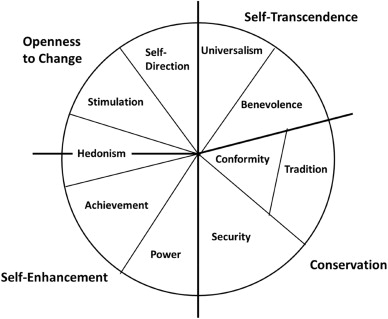
\includegraphics{TenValues}   
    \caption[The ten values from \textit{the Schwartz Theory of Basic Values}.]{The ten values from \textit{the Schwartz Theory of Basic Values}: self-direction, stimulation, hedonism, achievement, power, security, conformity, tradition, benevolence, and universalism. The circle is divided into four categories: openness to change and conservation, which represent the contradictories independence and obedience respectively, and self-transcendence and self-enhancement, which represent the contradictories interest in welfare of others and interest in welfare of oneself respectively. Values that work towards similar goals are placed in the same category \citep{schwartz2012overview}.}
    \label{fig:TenValuesSchwartz}
\end{figure}

\subsection{The Schwartz Value Survey}
In order to figure out how people prioritised their values, a survey was made by \citet{schwartz2012overview}. The survey made personality related statements and the participants answered how well the statement fitted their personality. Based on the results each of the ten values are assigned with a numerical value indicating how important that value is to the participant. The exact numerical value of the values is not what is important, it is their importance in relation to one another that matters. Normalisation is used on the ten values to scale them. 

The survey was answered by people from all over the world with many different backgrounds. A pattern in the prioritising of the values was found. It was found that benevolence, universalism, and self-direction were the most important values, while power, stimulation, and tradition were the least important ones. Almost all nations in which the study was conducted had these results. According to Schwartz, this indicates that the way people work and the way people are affected by society is quite similar in many different cultures.

%%%%%%%%%%%%%%%%%%%%%%%%%%%%%%%%%%%%%%%%%%%%%%%%%%%%%%%%%%%%%%%%%%%%%%%%%%%%%%%%%%%%%%%%%%%%%%%%%%%%%%%%%%%%%%%%%%%%%%%%%%%%%%%%%%%%%%%%%%%%%%%%%%%%%%%%%%%%%%%%%%%%%%%%%%%%%%%%%%%%%%%%%%%

\section{Graph Theory}
In recent years, a few papers have presented language game models with structured networks. \citet{lipowska2011naming} used a lattice to simulate a social graph, while others have incorporated social structures into their models \citep{lekvam2014co, gong2004computational}. This section will present discrete graphs, some of their features and how they are used in social networks.

A discrete graph is a discontinuous graph where the $x$-values of its function is limited to specific intervals, for example integers. This makes the graph consist of points, and not a line like a continuous graph. These points are usually referred to as vertices. The vertices in a discrete graph are connected with edges. These edges can be associated with a weight representing the cost between two vertices or not weighted, which essentially is the same as weighting all edges with the same value. In a discrete graph cities may be represented as vertices, and the roads between them as edges. The weight of the edges between cities could represent travel time or distance between the cities. If it is possible to travel both ways along an edge, the edge is called an \textit{undirected edge}. Otherwise, if it is only possible to travel in one direction along the edge, like a one-way driven street, it is called a \textit{directed edge}. A directed graph can have up to two edges between a vertice pair, while an undirected graph can have up to one edge between a vertice pair. Figure~\ref{fig:graph} shows an example of a directed and a undirected graph. Unless otherwise specified, the graphs presented in this thesis will be undirected.

A neighbour of a vertice, $v$, in a graph is another vertice which is connected to $v$ by an edge. The number of neighbours a vertice has is called the degree of the vertice. The density of a graph, $\mathrm{DENSITY}(G)$, is the number of edges in the graph $G$ divided by the theoretical maximum edges of $G$, $\mathrm{MAX}_\mathrm{edges}(G)$. In an undirected graph $G_\mathrm{undirected}$, with vertices $V$, the maximum number of edges are
\begin{equation}\label{eq:maximumEdges}
\mathrm{MAX}_\mathrm{edges}(G_\mathrm{undirected}) = \frac{V  (V-1)}{2}
\end{equation}

Using the definition of the density of a graph from above together with Eq.~\eqref{eq:maximumEdges}, the graph's density becomes
\begin{equation}\label{eq:densityOfGraph}
\mathrm{DENSITY}(G_\mathrm{undirected}) = \frac{2 E}{V(V-1)},
\end{equation}
where $E$ is the number of edges. Figure~\ref{fig:undirectedGraph} shows an undirected graph with three vertices: A, B and C. Vertices A and B have a degree of 1 since they have one neighbour each, while vertice C has a degree of 2 since it has two neighbours. By using Eq.~\eqref{eq:densityOfGraph}, the density of the graph becomes $2\cdot2 / (3\cdot2) = \frac{2}{3}$.

\begin{figure}[htbp]
    \centering
    \hfill
    \subfigure[\todo{FJERNE}Directed graph.]{\includegraphics[width=0.4\linewidth]{Directed_graph}\label{fig:directedGraph}}
    \hfill
    \subfigure[\todo{FJERNE}Undirected graph.]{\includegraphics[width=0.4\linewidth]{Undirected_graph}\label{fig:undirectedGraph}}
    \hfill
    \caption[The difference between a directed and an undirected graph.]{An illustration of the difference between \todo{\subref{fig:directedGraph}} a directed and \todo{\subref{fig:undirectedGraph}} an undirected graph. The circles represent vertices and the straight lines, both with and without and arrow, represent edges.}
    \label{fig:graph}
\end{figure}

\acresetall
\section{Social Networks}
A social network is a discrete graph where each vertice is a person and the edges represent how strongly two people are connected. There are a lot of factors that affect social networks and how they evolve over time. Some of these factors are language, personalities, and the environment of the social network. Several computational models that simulate the evolution of social networks have been designed. \citet{lipowska2011naming} used a lattice where each agent was restricted to only communicating with its neighbours except its first dialogues which it had with its parents. This model obviously has many limitations, such as agents cannot gain or lose connections and the connections are not weighted. 
\citet{lekvam2014co} used a social network where the edges were weighted based on the communication between the agents. It was also possible to loose and gain connections. This social network is a better representation of the real world than Lipowska's lattice, but there are other factors than just having the same language that affect a social network, like the personalities of the people in the network.

%%%%%%%%%%%%%%%%%%%%%%%%%%%%%%%%%%%%%%%%%%%%%%%%%%%%%%%%%%%%%%%%%%%%%%%%%%%%%%%%%%%%%%%%%%%%%%%%%%%%%%%%%%%%%%%%%%%%%%%%%%%%%%%%%%%%%%%%%%%%%%%%%%%%%%%%%%%%%%%%%%%%%%%%%%%%%%%%%%%%%%%%%%%

%Et lite latex-triks: Latex kan holde styr på akronymene dine, som f.eks. GA, i fila backmatter/acronyms.tex. Her legger du inn akronymet og det fulle ordet. Når du skal bruke det i teksten skriver du bare backslash ac{GA}. Første gang det dukker opp i teksten vil det fulle ordet pluss forkortelsen i parentes dukke opp, e.g. genetic algoritm (GA), mens andre, tredje, osv. gang vil kun forkortelsen dukke opp GA. For du skal ikke definere hva forkortelsen er mer enn én gang. Og ved hjelp av dette holder latex styr på det for deg. Smart, ikke sant?

\section{Genetic Algorithms} \label{GAalgorithm}
A \ac{ga} is a search algorithm based on the Darwinian principle of biological evolution. Imagine that you got the job of optimising an exam schedule at a university so that every student could take their desired combination of courses and be pleased with the exam dates. This would be impossible for humans due to the large search space. There probably does not even exist a solution where every student is pleased. In problems without a guaranteed optimal solution and with a large search space, \acp{ga} perform well.

The general structure of \iac{ga} can be seen in Figure~\ref{fig:GA}. First, a population of solutions is made, and all solutions are tested through a fitness function, which evaluates solutions and returns a fitness value that reflects how fit the solution is. Then survival selection is performed by having the fittest individuals of the population, or the best solutions, survive while the rest of the population dies. The solution that each individual represents is defined by a set of parameters, often referred to as an individual’s \textit{genome}. The genome is often represented as a bit-string. New solutions are then created by having the surviving solutions combine their genomes into new genomes by crossover, see Figure~\ref{fig:Crossover}. When a new solution is made, it has a small chance of mutation, i.e. a small alteration of the genome of the solution. Then these solutions are tested, and once again the fittest individuals survive to the next generation and get to breed.

The flow of a general \ac{ga} looks like this \citep{michalski2013machine}:
\begin{enumerate}[noitemsep]
    \item \textbf{Initialisation:}\\Initialise a population of individuals with random solutions.
    \item \textbf{Evaluation:} \\Calculate the fitness of all individuals.
    \item \textbf{Termination clause:}\\While the highest fitness value in the population is smaller than the desired fitness value or the maximum number of iterations has not been reached, the following steps are performed:
    \begin{enumerate}
        \item \textbf{Parent selection:} Select which individuals to bring into the next generation based upon their fitness.
        \item \textbf{Recombination:} Probabilistically select two individuals based on their fitness and combine their solutions into two new solutions by using crossover.
        \item \textbf{Mutation:} Randomly select a few of the new individuals and let their genome mutate.
        \item \textbf{Evaluation:} Calculate the fitness of the new solutions.
    \end{enumerate}
\end{enumerate}


\begin{figure}[htbp]
    \centering
    \includegraphics[scale=0.7]{GA_flow}
    \caption[Flowchart of a general \ac{ga}.]{Flowchart of a general \ac{ga}. First a population is initialised with random genomes and the fitness of all individuals is calculated. As long as the highest fitness value in the population is smaller than the desired fitness value, the \ac{ga} loop is run: 1) the parents for the next generation are selected; 2) the genomes from the parents are combined by crossover to constitute the genomes of the offspring; 3) a mutation of the genome can occur; 4) the fitness of all individuals is calculated; and 5) if the highest fitness value in the population is higher than the desired fitness value, the loop is terminated, otherwise, the loop is run again.}
    \label{fig:GA}
\end{figure}

A \textit{fitness function} is a function that returns a value which gives information about how good a solution is. The fitness function of a \ac{ga} that tries to find the fastest route from one city to another would simply be the travel time of the required solution. Many problems do not have so clear objectives, or have several objectives that need to be weighted in a more complex manner.

A common issue when searching with a \ac{ga} is that if the problem at hand contains many local maxima and few global maxima, the algorithm is likely to get stuck in a local maximum because one solution is more likely to discover a local maximum than a global maximum. This solution will then often be the fittest in the population, and spread its solution to the following generations. It is called \textit{exploitation} when a good solution is spread to many agents. Exploitation allows the algorithm to perfect one solution, but it stops exploring other possibly better solutions. \textit{Exploration} is searching for new types of solutions, which is done through mutation and probabilistically choosing parents. 

One of the most common methods used in the parent selection phase is called \textit{tournament selection}. This method combines exploration, by having some randomness, and exploitation, by prioritizing the most fit individuals. First, $k$ individuals are chosen at random from all individuals. Then the individuals are sorted by their fitness, and given a rank, $r$, accordingly, i.e. the fittest individual is given $r=1$, the second fittest $r=2$, etc. Then each individual is chosen with a probability, given by
\begin{equation}
p(1-p)^r,
\end{equation}
where $p$ is a user-given probability, $0 < p < 1$, for choosing the fittest individual in a tournament. 

When two parents have been selected to mate, crossover is performed and two new individuals are created based on the parents' genomes. The most common form of crossover is performed by randomly choosing one point on the bit-string, and splitting each parent's genomes into two parts, A and B. One child receives part A from one parent and part B from the other parent. The other child receives the opposite parts. See Figure~\ref{fig:Crossover} for a simple graphic explanation of crossover. Mutation is performed on an individual with a user-given probability. Mutation is normally performed by simply flipping one bit in the bit-string.

\begin{figure}[htbp]
    \centering
    \includegraphics[scale=0.7]{crossover2}
    \caption[How crossover is used to create two offsprings from two parents with a genome represented by a bit-string.]{How crossover is used to create two offsprings from two parents with a genome represented by a bit-string. First, the genomes of the parents are divided into two parts at the same spot. Then the first part of the genome of the first parent is combined with the second part of the genome of the other parent to form the genome of the first offspring, while the first part of the genome of the second parent is combined with the second part of the genome of the first parent to form the genome of the second offspring.}
    \label{fig:Crossover}
\end{figure}
 
%%=========================================
\acresetall
%%=========================================
\chapter{State-of-the-art}\label{ch:LitteratureStudy}

In this chapter, a description of the computer simulations of language evolution, from \citet{lipowska2011naming, gong2004computational, munroe2002learning, lekvam2014co} will be presented. These four were chosen because they have contributed with new ideas and represent different approaches in the field of using computational models to simulate language evolution.   

\section{Lipowska, 2011}\label{sec:Lipowska}
Lipowska made a computational simulation, which used a naming game to model a non-structured language. A non-structured language is a language that has no grammar or compositionality. The objective of Lipowska's model was to illustrate the Baldwin effect. 

\subsection{Model}
Lipowska incorporates the naming game in her model, which means that every agent is equipped with its own vocabulary, which contains all words it has heard of. Each word in the vocabulary is associated with a weight, $w_{i}$. The weight of a word represents how successful the word has been in conversations for an agent. All agents in the model are placed in a \textit{lattice}. A random agent is chosen as the speaker, and with probability $p\in$ $[0, 1]$ it chooses one of its neighbours in the lattice as the listener. If a neighbour is not chosen as a listener, the agent dies. If a neighbour is chosen as a listener, the speaker then utters a word from its vocabulary, and the listener receives that word. Which word the speaking agent utters is decided by the weight of each word relative to the sum of all weights in its vocabulary, $w_{i} / \sum_{j} w_{j}$, where $w_i$ is the weight of word $i$ and $\sum_{j} w_{j}$ is the sum of all weights of the words in the agent's vocabulary. If the agent has no words in its vocabulary, it makes one up at random. If the vocabulary of the listening agent contains the spoken word, the conversation is considered a success. If the word is not in the listener's vocabulary, the conversation has failed. 

Both the listening and the speaking agent adjust the weight of their word after a conversation. If the conversation was a success, both agents increase the weight of the word according to their respective learnability variables. The learnability variable $ l \in [0, 1]$ is an alignment strategy. Alignment is a strategy that is supposed to bring their languages closer to each other \citep{steels2012experiments}. At the end of each generation, which consists of several conversations between agents, some agents die based on a probability set by the average weight in the agent's vocabulary and its age. A high average weight in an agent's vocabulary increases its fitness, whilst an agent loses fitness when it gets older. For example, if the fitness of two agents with different ages, but with the exact same average weight over their vocabularies, is compared, the youngest of the two will have the highest fitness. A young agent with a high average weight in its vocabulary is an optimal agent. A surviving agent may breed, and if it does, the offspring inherits the learnability of its parent with a certain probability. If the offspring does not inherit its parent's learnability value, it is randomly set.

\subsection{Results and Discussion}
The experiments that were performed with a small $p$ resulted in agents that did not evolve a common language. Only small clusters of agents created common languages. The value of $p$ was slightly increased for every simulation. When $p$ increased, the size of the clusters of agents slightly increased. When $p$ reached a certain threshold, almost all agents became a part of the same cluster. For each simulation, the communication success rate, $s$, was also calculated. $s$ is defined as the fraction of all successful communications over the total number of communication attempts. When $p$ got the value of about 0.23, the communication success rate increased rapidly. 

The results of the experiment show a correlation between communication success rate and average learnability. In Lipowska's model, the new individuals require learning to incorporate the communal language that the generation before used. By communicating with the parents, the new agents learn the language the parents used. Children with a high learnability will learn more quickly than the others. According to Lipowska, the model shows that learning can direct the evolution, which indicates that the Baldwin effect has an influence on language evolution \citep[Section 4]{lipowska2011naming}.

%%%%%%%%%%%%%%%%%%%%%%%%%%%%%%%%%%%%%%%%%%%%%%%%%%%%%%%%%%%%%%%%%%%%%%%%%%%%%%%%%%%%%%%%%%%%%%%%%%%%%%%%%%%%%%%%%%%%%%%%%%%%%%%%%%%%%%%%%%%%%%%%%%%%%%%%%%%%%%%%%%%%%%%%%%%%%

\section{Gong, 2004}\label{sec:Gong}
This section will present the word order regularity model, its results, and what was concluded in the paper by \citet{gong2004computational}. 

\subsection{Model}
Gong made a simulation of the evolution of compositional language  where agents converse about ``integrated events such as tiger is running'' \citep[Section 3]{gong2004computational}. The speaking agent makes utterances trying to explain what it perceives, while the listening agent tries to understand the utterance in accordance with partial information about the environment they are in. The language evolves from a simple holistic language into a compositional language, thereby replicating how the human language is thought to have evolved. A holistic language is a language where one utterance can be mapped to a concept, such as hunt, storm, or fire. Holistic languages are primitive and complicated sentences such as \textit{a storm is coming from the east soon and, therefore, we have to find shelter}, can be hard to communicate using a holistic language. A compositional language is what humans speak today. This type of language allows multiple concepts to be combined easily. In Gong's simulation, a holistic rule is a rule that can be mapped to a specific concept, while compositional rules can be combined into different meanings depending on the order they are presented.    

The language in Gong's model is a set of mappings between meanings and utterances, so called M-U mapping. Meanings are represented as predicate-argument structures. The predicates are actions, such as \textit{run}, and the arguments are the objects that the actions are performed upon. When several arguments are used together with a predicate, the order of the arguments decide their role. An agent's language is stored through three rules: lexical rules which are M-U mappings; syntactic rules which define the compositionality by describing the order to use lexical rules; and syntactic categories which contain sets of lexical and syntactic rules that are linked to each other. All syntactic and lexical rules have a strength which describes how likely they are to use their M-U mapping successfully. The lexical rules also have an association weight which describes how likely the rule is to be linked to the category it contains. For a more detailed explanation of Gong's compositional language see \citep[section 3.2]{gong2011simulating}.
%For example Hunt<tiger, deer> could have two meanings. The first argument is the agent, the one that performs the predicate. The second argument is the object that agent is performing the predicate upon. In this example, it means that the tiger is hunting the deer. Predicates with identical arguments are excluded from the model for simplicity. 
\begin{comment}
The agents can store knowledge through three rules:
\begin{enumerate}%[topsep=0pt,itemsep=1ex,partopsep=1ex,parsep=1ex]
   \item \textbf{Lexical rules:} are M-U mappings. A rule is activated if the rule fully or partially matches what the speaking agent uttered. A \# indicates that any object can be used in that place. \\
   Example: Hunt<tiger, \#>, indicates that tiger is hunting any object that is inserted instead of the \#.

    \item \textbf{Syntactic rules:} are the rules that control the compositionality. These rules define the order between two lexical terms. There are four types of ordering rules that define the ordering: before a word rule, after a word rule, surround a word rule, and between a word rule. ``''<<'' is the local order before, ''>>'' is after, $\bigtriangledown$ is surround, and $\bigtriangleup$ is between'' \citep[chapter 3.2]{gong2011simulating}.\\
    Example: Category 1 (S)<< Category 2 (V), means that category 1, the subject (S), is before category 2, the verb (V).

    \item \textbf{Syntactic categories:} are a set of lexical rules and syntactic rules that is linked to each other. This makes it possible to combine several rules with the same category. In this model, the syntactic categories represent the subject, the agent is the object, and the predicate is the verb.\\
    Example: Category 1 (S): List of lexical rules: Hunt<tiger, deer>, Category 1 (S)<< Category 2 (V). This category collects all rules that are connected to the subjects (S) of an utterance. 
\end{enumerate}
\end{comment}
%If a speaker does not have any lexical rules to describe a meaning, the speaker will randomly create an utterance and store this mapping as a holistic rule. In the beginning, many such rules will be created. The agents use pattern extraction to learn rules. If an agent extract identical meanings from the same rules repeatedly, compositionality will eventually emerge. 

Gong's model uses a \textit{random communication framework} \citep[section 3.4]{gong2011simulating}. Two randomly chosen agents perform many transactions of utterances. The speaker begins by randomly selecting a meaning to produce. The speaker then goes on to activate the lexical rules and the syntactic categories that regulate the rules to form a sentence. The speaker then calculates the set of winning rules, and builds up the sentence using these rules. If the speaker does not have enough knowledge to express the meaning, then random creation of rules occur.
The listener receives the utterance from the speaker together with an \textit{environmental cue}. The cue contains partial information about the environment. The lexical rules that fully or partially match the sentence received are activated. A candidate set consisting of possible ways to understand the input gotten from the speaker is created.  
\begin{comment}
\begin{enumerate}
    \item If the cue and some set of the rules match perfectly, they are combined into a candidate set.
    
    \item If the rules and the cue do not make a perfect meaning, but the constituents of the rules match the constituents in the cue, then they are combined into meaning. Gongs example of this is as follows: The linguistic rule interpreted from the sentence is Chase<tiger, \#> and the cues meaning is Chase<tiger, sheep>. These rules do not match perfectly, but they will be combined into the meaning Chase<tiger, sheep>, which is the meaning of this candidate set.
    
    \item If none of the linguistic rules from the sentence received can be combined with the cue, then the cue becomes a candidate set. Gongs example here is: Say we have the rule Chase<tiger, sheep> from the utterance, but the cue gives the rule Fight<tiger, sheep>. These rules can not be combined, and therefore, the cue becomes the meaning.
\end{enumerate}
\end{comment}
The listener calculates the strength of each candidate set. The rules of the strongest set is then used to interpret the received sentence. If the strength of the strongest set exceeds a certain threshold, the M-U mapping is added to the listener's buffer and positive feedback is given to the speaker. Then both agents reward or retract strength from their rules according to how the communication went. It is never checked whether the agents actually ended up with the same meaning.

\subsection{Results and discussion}
In total, 20 simulations with 6000 communication rounds were performed during each simulation. The simulations were performed with a population size of 10 and with 20 utterances per communication. During the first 100 rounds of communication, many holistic rules were created, but almost no compositional rules were formed. After 200 rounds, the number of holistic rules dropped, while many compositional rules were created. Throughout the first rounds of communication, holistic rules are the main resource for understanding utterances and cues. Very few agents share holistic rules, so a lot of the communication results in the agents not understanding each other. When compositional rules start appearing, a clear increase in the number of successful communications is observed. Once some compositional rules become shared among the agents, almost all communications are successful. It is also observed that while the rate of successful communications rise, the average amount of meanings that each agent can make increases. That fact that the agents can express many meanings and that the agents understand each other almost every time, indicate that a compositional language has appeared. 
Gong concludes that ``given some general learning abilities, such as pattern extraction and sequential learning, a communal language showing a certain degree of systematicity can emerge in a population of individuals'' \citep[chapter 6]{gong2011simulating}.

%%%%%%%%%%%%%%%%%%%%%%%%%%%%%%%%%%%%%%%%%%%%%%%%%%%%%%%%%%%%%%%%%%%%%%%%%%%%%%%%%%%%%%%%%%%%%%%%%%%%%%%%%%%%%%%%%%%%%%%%%%%%%%%%%%%%%%%%%%%%%%%%%%%%%%%%%%%%%%%%%%%%%%%%%%%%%%%%%%%%%%%%%%%

\section{Munroe \& Cangelosi, 2002}\label{sec:Munroe}
Munroe and Cangelosi's simulation \citep{munroe2002learning} studies how learning during the lifetime of an individual affects language evolution.

\subsection{Model}
 In their simulation an agent is supposed to identify whether a mushroom is edible or not based on an 18-bit representation of the mushroom's features. The world contains three sorts of edible mushrooms and three non-edible ones. The three edible mushrooms require their own type of preparation in order for the mushroom to be edible (wash, cut, squash). An agent walks around in a grid-based world for 50 steps. In order to see that an agent could perform in different environments, each agent completed 20 different worlds during one generation. The fitness of an agent is calculated by awarding 1 point every time an agent performs the correct preparation of an edible mushroom. On some of the simulations, it was intended to simulate a learning cost. The learning cost would subtract 1 point if a non-edible mushroom was eaten. \Iac{ffnn}  was used by the agents to classify the mushrooms. \Iac{ffnn} is the simplest form of \ac{ann}, where all signals are distributed in one direction, forward. Other \acp{ann}, such as recurrent neural networks can send signals backwards in the network creating cycles \citep{jain1996artificial}.

The simulation has two stages. The first stage lasts for 300 generations with a population of 100 agents. All agents try to eat as many edible mushrooms by analysing the mushroom's features. After all agents have completed their 20 worlds, the 20 best performing agents become parents of the next generation. The 20 agents make 5 copies of themselves where 10 \% of their weights are mutated. The model was set up so that cultural variation could be simulated by applying noise before the 20 best agents were selected.

The second stage lasts for 100 generations and now the agents are allowed to communicate with each other. The 20 best performing agents are carried over to the next generation and act as teachers. 90 \% of the time the agents will not have access to the features of the mushroom, but they will receive an input from their parent telling them what kind of mushroom they are observing. The other 10 \% of the time the agents have access to both the features of the mushroom and the input from their parents before deciding what action to take. After this, the child is provided with the features of the mushroom and generates its own description of the mushroom. Using backpropagation, the child corrects its output based on the parent's description of the mushroom. Finally, the child imitates the description of the parent by only taking the parent's description as input, trying to reproduce the parent's description as output, and performs backpropagation.

\subsection{Results and discussion}
Ten experiments were ran with different population sizes. At the end of the first stage (300 generations), eight of the experiments solved the game perfectly, by avoiding all non-edible mushrooms and preparing all the edible ones correctly. The agents reached the optimal fitness of 70 at approximately generation 150.
Those eight experiments went on to the second stage of the simulation. Seven of these managed to solve the game by combining the occasional input from the environment with the linguistic input from the parents. During the second stage, the agents reached a fitness level of 70 after only 90 generations. 
Four of these experiments created compositional languages. The language created was compositional because the first symbols were always related to the action and the last symbols were associated with the type of mushroom.
%The languages consisted of symbols for the actions approach and avoid to tell the agents whether it was edible or not. The other signals were linked to the food types. 

Experiments with the cultural variation and learning cost parameters at different values were performed. The idea behind varying the cultural variation and learning cost was that it is assumed that the Baldwin effect will be strongest when the cultural variation is low and the costs of learning outweigh the benefits.

%\subsection{Conclusion}
It was concluded that a Baldwin effect was observed in these experiments. \citeauthor{munroe2002learning} found that with a learning cost and a changing environment, some individuals learned the language quicker than others. It was also found that when the learning environment was fixed, specific behaviours got stored in the genome. When the cultural variation was set to 0, i.e. no noise when selecting the fittest agents, even the language structure itself could be built into the agent's genome.

This experiment indicates that the theory that individuals can inherit capabilities that will help learn features more easily might be valid. In order to understand exactly how these mechanisms work more research is needed.

\section{Lekvam, 2014}
Lekvam's simulation \citep{lekvam2014co} was based on the \ac{ga} framework, that was explained in section \ref{GAalgorithm}, and inspired by the model by \citet{lipowska2011naming} and the work on social networks done by \citet{quillinan2006social}. \citeauthor{lekvam2014co} also had a goal that it should be easy to add extensions to his model.

\subsection{Model} 
\citeauthor{lekvam2014co}'s model has two processes evolving at the same time, a social structure and a language. The agent's goal is to acquire a social network, which is accomplished by having successful conversations with other agents. The fitness of the agent is a combination of its connections and its age using the formula
\begin{equation}
    \mathrm{fitness} = [\exp(0.02 \cdot N_\mathrm{relations}) - 1] \exp(-0.05 \cdot t),
\end{equation}
where $N_\mathrm{relations}$ is the number of connections an agent has and $t$ is the age of the agent. The more relations an agent has, the higher fitness it has, while the agent's age negatively influences its fitness. Lekvam argues that this is a good measurement of fitness because how well an agent can communicate will affect its ability to reproduce. 

When an agent acquires $z$ connections, it will stop reaching out to others, but focus on keeping the connections it has. Other agents with less than $z$ connections can still contact it, meaning that having more than $z$ connections is possible. All connections in the social network are weighted. A successful conversation increases the weight by $1.0$, while an unsuccessful one subtracts $0.5$ from the weight. 

The genome of the agents consists of four genes:
\begin{enumerate}
    \item \textbf{Extraversion} is the probability of searching one layer out in the network for new friends, given that the agent has less than $z$ connections.
    
    \item \textbf{Teach child} is the probability that the parent will be the first to speak to its child. If both of the parents have high values, it is very likely that the parents will speak to the child first.
    
    \item \textbf{Lexicon limit} is the maximum size of an agent's vocabulary. If the agent learns a new word, but its vocabulary is full, the lowest weighted word is removed.
    
    \item \textbf{Speech ability} is the probability that an agent will not randomly invent a word even though it has chosen one from its vocabulary to utter. If the probability of speech ability is high, there is a high chance that the chosen word is uttered.
\end{enumerate}

When deciding which agents that will go through to the next generation, tournament selection is used. When the set of surviving agents has been selected, they breed. Each agent chooses a partner close to it in the network and then crossover is used to combine their genes. The child has a small probability to mutate. 

\subsection{Results and discussion}
The simulations were conducted with 200 generations per simulation, a population of 1225 agents per simulation, and 5 conversations per agent per generation. Seven versions of the simulation were ran. This summary will only present the results from simulation 1, which was the main simulation of the thesis. 

It was observed that the first relationship almost all newborn agents had, was with their parents. This is an easy way to make connections for the agents. The agents quickly found out that reaching far out into the social network was beneficial. Since the agents' method of acquiring more than $z$ connections was to have other agents contact them, reaching far out will increase the chances of other agents reaching out to you. The population very rarely reached full consensus. Most of the time two or three languages remained when the simulation was completed. The final social network reflects this result, as the agents usually create two or three groups.

Lekvam discusses that his model might have too many flaws to conclude anything certain. Using a naming game might not be the best way of modelling signals being mapped to meaning. He also mentions that the fitness function used in the model might not be realistic enough. However, he does conclude that he believes that the methodology used has ``a great potential''.

%%%%%%%%%%%%%%%%%%%%%%%%%%%%%%%%%%%%%%%%%%%%%%%%%%%%%%%%%%%%%%%%%%%%%%%%%%%%%%%%%%%%%%%%%%%%%%%%%%%%%%%%%%%%%%%%%%%%%%%%%%%%%%%%%%%%%%%%%%%

\section{Comparison of the Four Models}
All four language evolution models presented utilise language games. These four language game models are simplifications of how humans communicate while maintaining the essence of why humans communicate in the model. the essence being that in order for the human species to survive, humans need to communicate and understand each other. Language games replicate how an individual is able to learn a language through having each person evolve a personal language based on communication with other people. The language game models made by \citet{lipowska2011naming} and \citet{lekvam2014co} both used a naming game. The two other language games presented in the literature study were a spatial naming game and a signalling game. 

The spatial naming game and the signalling game incorporated word order regularity because the models studied how a compositional language could evolve, and how a population may reach a consensus over a compositional language. These models became complicated because they studied something as complex as the evolution of a compositional language. 

The two naming game models presented were simpler than the spatial naming game and the signalling game because both naming games used a holistic language. The naming game was used to study how individuals in a population could reach a consensus concerning what utterance to use to name an object. These models studied how cultural learning has an effect on language evolution, and to do that, compositional models were not needed. 

An agent’s language changed based on conversations in all the models, so how an agent decided whom to converse with had a substantial effect on how a language evolved. Gong’s model \citep{gong2011simulating} used randomly chosen speakers and listeners, and hence, the agents did not get to decide their listener, which could have made the language evolve unnaturally. However, in the model by \citet{munroe2002learning}, the parents spoke to their children, which was an improvement compared to Gong’s model, but the agents did not get to choose conversational partners by themselves.

In the model by \citet{lipowska2011naming}, the agents were set in a lattice world, with newborn agents being placed between their parents and two other agents in the lattice. This meant that every agent was directly connected to four other agents, and like in \citeauthor{munroe2002learning}'s model an agent would conduct most of its conversations with its parents while they were still alive. It also meant that an agent had a set amount of edges, and lacked the ability to establish a connection to others. The edges were not weighted, meaning that all relationships between the agents were equally strong in this model. Lipowska gave all agents the ability to choose their own conversational partner, but the way a social network was represented had its limitations. 

In the model by \citep{lekvam2014co}, which was inspired by \citet{lipowska2011naming} and \citet{quillinan2006social}, each agent could acquire new connections by contacting other agents. In contrary to \citeauthor{lipowska2011naming}'s model, agents could lose edges if several conversations between two agents were unsuccessful in \citeauthor{lekvam2014co}'s model. Each edge was weighted so that not all relationships were equal in this model. \citeauthor{lekvam2014co} made a social network in which the agents decided who to converse with, unlike in \citeauthor{gong2011simulating}'s model which randomly chose speakers and listeners. It could be someone the agent knew or it could contact a new agent. What was missing from this model was how agents decided whom to converse with, which was done randomly, and that both agents had the same degree of connection towards one another. 

In all the models, the fitness of an agent is supposed to be an image of how well that agent performs in a specific environment. In both Lekvam’s and Lipowska’s model, the fitness of an agent was supposed to reflect the agent’s ability to be understood by others. Lipowska used a fitness based on the average weight of the words in an agent’s vocabulary and its age. The average weight over the vocabulary described how well an agent was understood, but it did not describe how many agents that understood the agent. 

Lekvam used a fitness based on the number of edges of an agent and the agent’s age. The number of edges described how many other agents that understood the agent, unlike \citeauthor{lipowska2011naming}'s fitness function. However, the fitness function did not describe to what degree the agents understood each other. In order to do that, the fitness function would have required the weights of the social network to be used. Lekvam’s fitness function did not reward having strong edges. If one agent had ten edges, with weights less than $0.1$, while another agent had eight edges with weights more than $0.8$, the agent with the strongest weights should be compensated for having strong connections, in terms of an increased fitness. Both models used the age of an agent as well, which represented that the older an agent became, the more likely it was to die. 

\citet{munroe2002learning}, on the other hand, used a very different fitness function which was based on how well an agent acted in an environment. How well an agent performed was directly correlated to how well the agent understood the input it got from its parents, and so the fitness function reflected how an agent was able to understand other agents. The language was not used as a part of the fitness directly, a separate world was created where an agent's ability to understand language was tested. This was a clever method which tested how an agent learned the language of its parents.


%%=========================================
\acresetall
%%=========================================
\chapter{Methodology}\label{ch:Chapter4}

This computational model is based on Lekvam’s model, adding personalities based on Schwartz' 10 values model \citep{lekvam2014co, schwartz2012overview}. This chapter will also present a new method for choosing a listener, calculating the weights in the social network, and a new fitness function.

The model use a genetic algorithm which simulate the evolution of language and social networks over time. Tournament selection is used as parent selection. In tournament selection, a pool of random agents are chosen. Then the agents are sorted based on their fitness. The probability of an agent being chosen is,
\begin{equation}
    \label{eq:TSelect}
    P_{parent} = p ((p-1)^{i})
\end{equation}
where $i$ is a counter starting at zero, and $p$ equals the probability of the fittest agent in the pool being chosen as the parent. Turnover selection is performed by randomly choosing $k\%$ of the population into a pool. Then, the $n\%$ least fit agents of that pool do not survive until the next population. 

Personalities are added into the model in the form of an agent’s genome. The genotype of an agent consists of one number between $[0, 100]$ for each of the ten values from Schwartz’s model. The values can not be randomly initiated because some of the values describe relatively equal goals, while some other values are contradictory. If two contradicting values both have a high value, the goals of that person would contradict each other. So, in order to ensure the validity of the relations between the ten values, all values can not be created randomly. In figure \ref{fig:TenValuesSchwartz}, the values are divided into four groups. Values within a group are related and should have numerical values close to each other. While values on the opposite side of the circle should have opposite numerical values. In this model, the validity of the relations between the values are kept by randomly setting the self direction and achievement value. Values in the same quadrant are set by using this formula:

\begin{equation}\label{eq:valuesInSameQuadrant}
V_{i} = \frac{\mathrm{random}(0, 20)}{100} \ast V_{i-1},
\end{equation}
where $V_{i}$ is the number associated with value $i$, $V_{i-1}$ is the number associated with the value counter clockwise of $V_i$ in the circle, and $\mathrm{random}(0, 20)$ is a random integer in the interval $[0, 20]$. Security and benevolence is set based on the opposite value using the formula:
\begin{equation}\label{eq:valuesInOppositeQuadrant}
V_{i} = \frac{\mathrm{random}(1, 20)}{100} \ast (100 - V_{\mathrm{opposite}}).
\end{equation}

The other values in the quadrants with security or benevolence is set based on the formula \ref{eq:valuesInSameQuadrant}. Hedonism is split between two quadrants and it is therefore calculated based on the two values next to it in figure \ref{fig:TenValuesSchwartz} through this formula:
\begin{equation}\label{eq:hedonism}
V_{i} = \frac{\mathrm{random}(1, 20)}{100} \ast \frac{V_{i-1} + V_{i+1}}{2}.
\end{equation}

The values of the genome is then normalised, representing the individual’s personality and phenotype. A newborn’s genotype is made using crossover from two parents genotypes, and the new genotype has a small probability of mutation. Mutation is conducted by randomly altering one value in the genotype. Each agent have a vocabulary similar to the vocabulary used in Lekvam’s model. The vocabulary consists of the utterances an agent has heard or created. Each utterance have a corresponding weight describing how successful the utterance has been in past conversations.     

The social network in the model is represented by a weighted discrete graph, where the vertices represent the agents, and the edges represent the connections between the agents. If a dialogue is successful, the weight of the edge between the two agents increases and if it was unsuccessful the weight decreases. An edge gets added a weight of $1$ if the dialogue is successful and $0.5$ is subtracted if the dialogue was unsuccessful. This method of calculating the a weight allows the language of the agent to affect the weight of the edge.
 
The fitness function used is made to represent how well an agent communicates with the members of the community, as well as how the agent’s personality fits in with the group. An agent's ability to communicate was projected into the social network because the weights were adjusted based on an agent’s ability to be understood. The personality of the agents determines how good it is at learning a language, how extrovert it is, and whether it cares about its children. The fitness function also take into account the age of the agent. The fitness function is,

\begin{equation}\label{eq:Fitness}
\text{Fitness} = \Big( e^{\alpha \sum_{i=1}^{N}{W_{i}}}-1 \Big) \ast \Big( e^{\beta N_{W_{i\geq \text{constant}}}}-1 \Big) \ast \gamma e^{-0.05 \text{age}},
\end{equation}

where $W_{i}$ is the weight of an agent, $N$ is the total number of vertices in the network, $W_{\text{max}}$ is the strongest weight in the network, and $\alpha, \beta, and \gamma$ are constants adjusting the three parts of the fitness function. The first part calculates the sum of all weights of an agent to display how strongly it connects to others. The second part calculates how many agents with a minimum strength in connection the agent has a connection with. The third part provides an agent with less fitness the older it becomes. These three functions combined display the agent’s fitness in the society. It takes into account the number of connections it has, the strength of the connections, and its age.

When an agent chooses a listener, the agents social network and personality is used. An agent can either be extrovert or introvert, based on its values. The positive extrovert value is achievement; people often seek recognition for their achievements. An achievement no one knows about, is not worth anything. The negative value is conformity; restraint from doing certain actions because one is scared of the consequences. People who value this high think a lot about consequences and might be careful in social settings because of it. Each of these values were taken from an agent’s genome and is therefore in the interval $[0, 100]$. Based on these values, this formula describes the probability of an agent reaching out to agents that it does not already have a connection with,

\begin{equation}\label{eq:chooseListener}
P = \parentheses{\frac{\sum \text{extrovert values} + (100 - \sum \text{introvert values})}{200\ast C}}/100,
\end{equation}

where $C$ is a constant, between $[0.0, 1.0]$, which forces all individuals to have a tendency towards introvertedness. People tend to have more conversations with people they already know, so skewing the probability towards introvertedness seems reasonable. The first conversations a newborn has might be with its parents. The probability of having dialogues with parents is equal to the normalised value of the security value in the genome. Each parent will conduct three dialogues each and the newborn will function as the listener in all these conversations. If the speaking agent decides to act introvertly, the probability of contacting one specific agent is related to the weight between the agents:
\begin{equation}\label{eq:intrvertListener}
P_{i} = \frac{W_{i}}{\sum_{j=0}^{N}{W_{j}}},
\end{equation}
Where $N$ is the number of edges the agent had, and $W_{j}$ is the weight of an edge. If the agent decides to be extrovert, it randomly chooses an agent from the population to contact.

Agents also altered their personality based on who they communicate with. After a conversation, both agents altered their values using this formula,

\begin{equation}\label{eq:PCR}
\text{Personality change rate} = \parentheses{\frac{\Delta \text{Value} \ast \text{isSuccess}}{\text{age}}}\ast C,
\end{equation}

where $\Delta \text{Value}$ is the difference of a specific value in the two agents' genomes, $\text{isSuccess}$ is a boolean which ensures that the personality is not changed if a conversation is unsuccessful, and $\text{age}$ is the number of generations the agent has lived. After this is calculated for all values in the genome, it is normalised again.

One conversation is conducted by the speaker uttering a word from its vocabulary. The probability of a specific word from the vocabulary being uttered is:

\begin{equation}\label{eq:chooseWordprob}
P_{i} = \frac{W_{i}}{\sum_{j=o}^{N}W_{j}},
\end{equation}

where $W_{i}$ is the weight of word $i$ in the vocabulary, and $\sum_{j=o}^{N}W_{j}$ is the sum of the weights of all words in the vocabulary. If the speaking agent has an empty vocabulary, it invents a new word. If the listener has the utterance in its vocabulary, the conversation is redeemed as a success, and the weight of the edge in the social network is updated, the personality is altered, and the weight of the word in the vocabulary is changed for both agents. If the listener did not have the word in its vocabulary, the conversation is a failure, and the weight of the edge in the social network is updated for both agents. The speaking agent decreases the weight of the word in its vocabulary, while the listener adds the word into its vocabulary. None of the agents' personalities are changed when the conversation is unsuccessful.

%%=========================================
\acresetall
%%=========================================
\chapter{Results}\label{ch:Results}

This chapter will present the results gathered through seven experiments using the computational model presented in the previous chapter.

\section{Parameters}
Table \ref{tab:params} displays the parameters, the base values used in the main experiment, and a short explanation of each parameter. In a given experiment, the value of a parameter can be assumed to be the value associated with it in table \ref{tab:params}, unless no other value is specified.    

\begin{table}[htbp]
    \centering
    \caption[The parameters in the model.]{Table of the parameters in the model.}\label{tab:params}
    \begin{tabu} to 1.0\textwidth { X[1,c] X[1,c] X[5,p] }%{| c | c | p{0.8\linewidth} |} 
         \hline
         \rowfont\bfseries
         Parameter & Value & Description \\ 
         \hline
         a & 1000 & Number of agents in the population. \\ 
         g & 100 & Total number of generations the simulation will last for. \\

         d & 1 & Number of dialogues per agent per generation. \\

         k & 0.9 & $(k \ast 100 )\%$ of the population is randomly chosen into the survival selection pool. \\

         n & 0.5 & The $(n \ast 100 )\%$ fittest agents in the pool survive to the next generation. \\ 

         m & 0.02 & Probability of mutation. \\

         c & 0.5 & The constant which affects how extrovert agents can act. \\
         $\delta$ & 3 & Constant related to the probability of a child conducting its first dialogues with its parents.\\
         
         $\epsilon$ & 0.2 & Probability in the parent selection pool is $(1-\epsilon)$.\\ 

          $\alpha$ & 0.2 & Constant related to the fitness function part which concerns an agent's weights.\\

          $\beta$ & 0.12 & Constant related to the fitness function part which concerns an agent's edges. \\

         $\gamma$ & -0.05 & Constant related to the fitness function part which concerns an agent's age. \\
         
         $\Theta$ & 0.5 & The minimal strength of the edge for it to be counted in the part of the fitness function that concerns the agent's edges.\\
         \hline
    \end{tabu}
\end{table}

\section{Experiments}
This section will present seven experiments. The experiments were conducted in the order in which they are presented. The first experiment represents the main results and the foundation for all experiments performed after it. The next two experiments tested what happens when the population increases or decreases. The fourth experiment was performed with an increased amount of dialogues per generation. The results from the third experiment lead to a hypothesis which was tested in the fifth experiment through lowering the probability of parent-child dialogues. The hypothesis will be presented in the discussion of the results. Experiment six tested how altering the turnover affects the evolutionary processes in this model. The last experiment added a probability for agents to invent a new word even though their vocabulary is not empty.

In several of the experiments, some results were not included. The results not included were deemed as unimportant for the discussion in this thesis. These results can be seen in Appendix \ref{AppendixA}.

\subsection{Experiment 1 - Main results}
The main experiment was conducted with the exact values from table \ref{tab:params}. See Figures \ref{fig:exp1.0}, \ref{fig:exp1.1}, and \ref{fig:exp1.2} for the graphs related to this experiment.

The average fitness of the agents greatly increased during the first $40$ generations, and then the average fitness stabilised at about $0.85$, as seen in Figure~\ref{fig:exp1.0}\subref{fig:Fitness1}. The average degree of the agents also increased a lot during the first $40$ generations, eventually stabilising at an average of about $10$ edges per agent, as seen in Figure~\ref{fig:exp1.0}\subref{fig:Degree1}. 

Figure~\ref{fig:exp1.1}\subref{fig:Genes1} shows how the speaking to parents probability, learning rate, and extrovert probability evolved. The easiest method for a newborn agent to acquire connections was through dialogues with its parents, and the probability of that happening was slowly increasing during the entire simulation. The learning rate increased a lot during the first $20$ generations. After the first $20$ generations, the learning rate slowly increased during the remainder of the simulation. The extrovert probability increased during the first three generations, and then decreased to about $5\%$, indicating that agents who focused on gaining strong relationships gained a better fitness than extrovert agents with many weak relationships.  

The graphs describing the percentage of successful dialogues, as seen in Figure~\ref{fig:exp1.1}\subref{fig:succDia1}, number of unique highest ranked words in the vocabularies, as seen in Figure~\ref{fig:exp1.1}\subref{fig:uniqueWords1}, and average number of words in a vocabulary, as seen in Figure~\ref{fig:exp1.1}\subref{fig:Vocabulary1}, all tell the same story. In the beginning there were many words, all agents had large vocabularies, and few dialogues were successful. The number of unique words decreased substantially during the first $10$ generations, then at generation $62$, the population reached consensus. Consensus means that all agents had the same word as their highest weighted word. The graph which display the percentage of successful dialogues quickly reached $70\%$, then percentage gradually rose for the remainder of the simulation, ending at $90\%$. The average vocabulary size increased during the first generations, and then decreased until generation $60$, ending at an average of slightly more than one.

The figures displaying the social network at generation $5$, $20$, $40$ and $100$ only include the agents with a connection, which explains why the number of nodes is not equal in all four figures, and why there is a discrepancy between the social network and the graph displaying the average degree per agent. The farther an agent is away from the centre of the social network, the fewer edges it has. The nodes closest to the centre are the ones with the most edges. At generation $5$, most of the nodes seemed to have two or three connections each, as seen in Figure~\ref{fig:exp1.2}\subref{fig:exp1SN5}. By generation $20$, the number of unique words had gone down and many of the agents had acquired several connections, as seen in Figure~\ref{fig:exp1.2}\subref{fig:exp1SN20}. The network at generation $20$, seemed to be more polarised than it was at generation $5$. Some agents had many connections, while a lot of agents had only one or two connections. At generation $40$, the social network had become even more polarised, as seen in Figure~\ref{fig:exp1.2}\subref{fig:exp1SN40}. The agents in the centre had gotten more connections, while the agents outside of the centre still had one or two edges. At generation 100 most of the population with connections had several connections, as can be seen by the high density of edges at the centre of the figure, as seen in Figure~\ref{fig:exp1.2}\subref{fig:exp1SN100}. There were still a select few agents with one or two edges, but those were by far in a minority.

\begin{figure}[htbp]
    \centering
    \subfigure[]{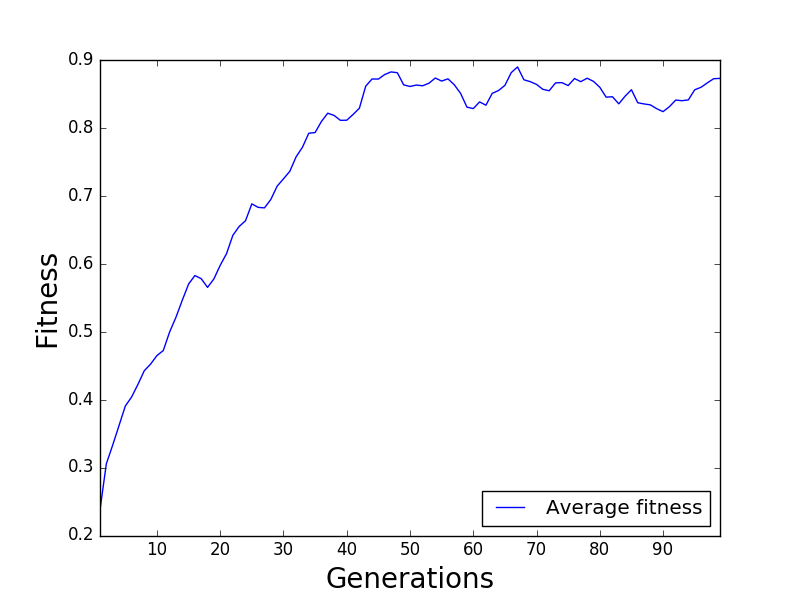
\includegraphics[width=0.49\linewidth]{fig/Results/Exp1/Fitness1}\label{fig:Fitness1}}
    \hfill
    \subfigure[]{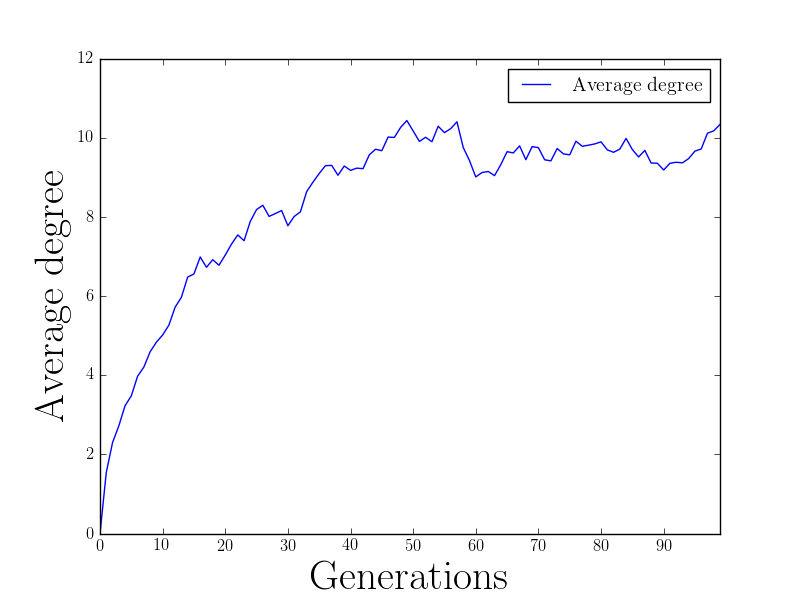
\includegraphics[width=0.49\linewidth]{fig/Results/Exp1/Degree1}\label{fig:Degree1}}
    \caption{Results from experiment 1. \subref{fig:Fitness1}: the average fitness and \subref{fig:Degree1}: the average degree.}
    \label{fig:exp1.0}
\end{figure}
\begin{figure}
    \centering
    \ContinuedFloat
    \subfigure[]{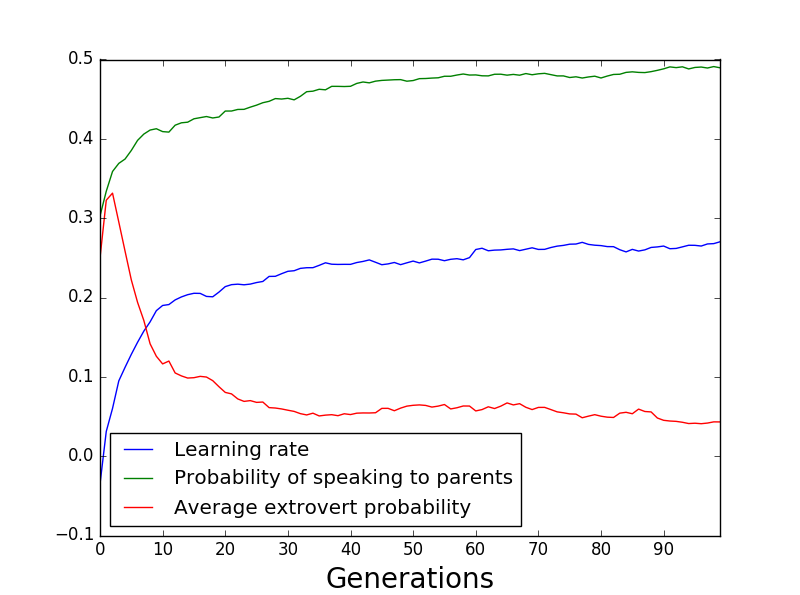
\includegraphics[width=0.49\linewidth]{fig/Results/Exp1/Genes1}\label{fig:Genes1}}
    \hfill
    \subfigure[]{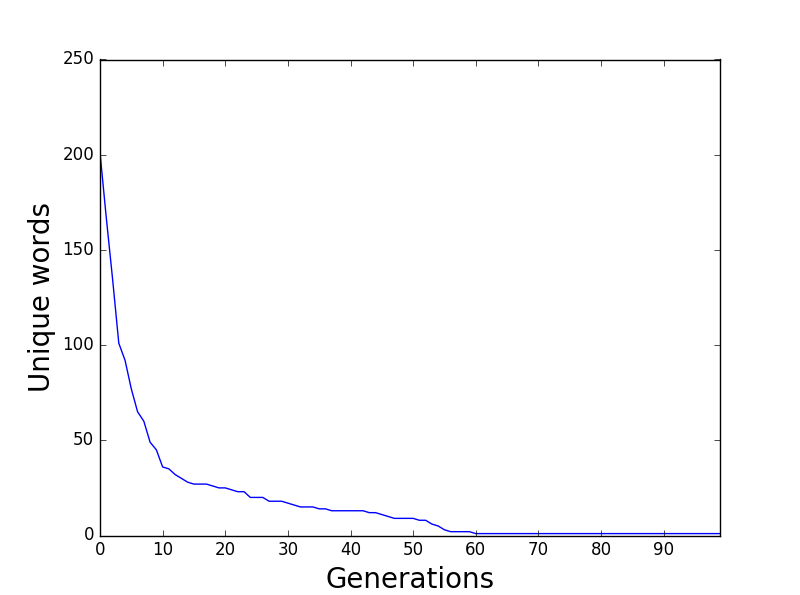
\includegraphics[width=0.49\linewidth]{fig/Results/Exp1/UniqueWords1}\label{fig:uniqueWords1}}
    \par \bigskip
    \subfigure[]{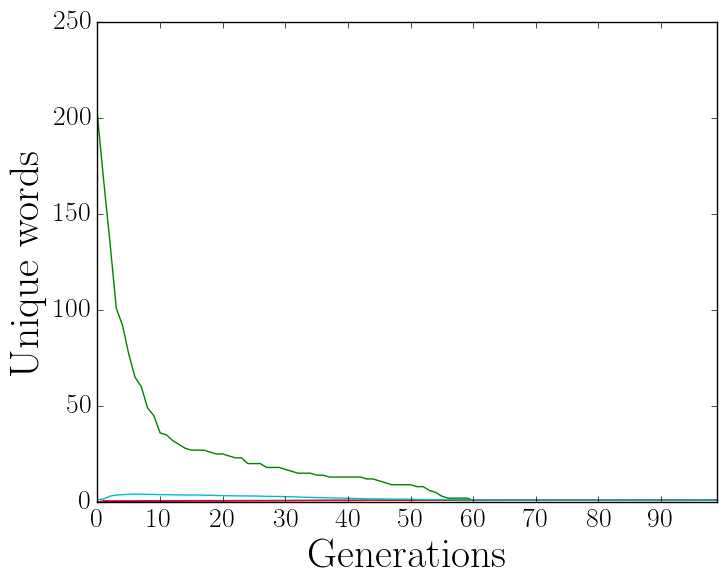
\includegraphics[width=0.49\linewidth]{fig/Results/Exp1/Vocabulary1}\label{fig:Vocabulary1}}
    \hfill
    \subfigure[]{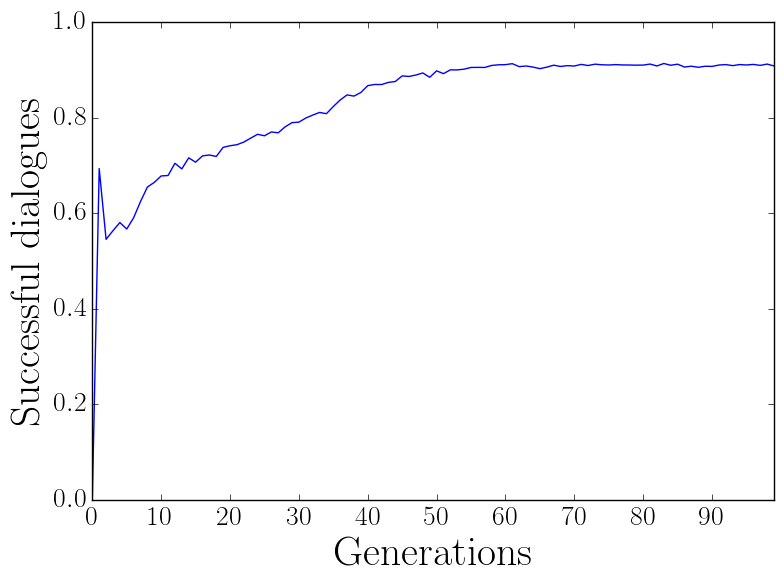
\includegraphics[width=0.49\linewidth]{fig/Results/Exp1/SuccDialogues1}\label{fig:succDia1}}
    \caption{Results from experiment 1. \subref{fig:Genes1}: the evolution of the traits from the genome. The three graphs in the figure are the green graph which is the average probability of conducting parent-child dialogues, the blue graph which is the average learning rate, and the  red graph which is the average probability of acting extrovertly. \subref{fig:uniqueWords1}: the number of unique highest ranked words in the population. \subref{fig:Vocabulary1}: the average vocabulary size. \subref{fig:succDia1}: successful dialogues divided by total number of dialogues.}
    \label{fig:exp1.1}
\end{figure}
\begin{figure}[htbp]
    \centering
    \subfigure[]{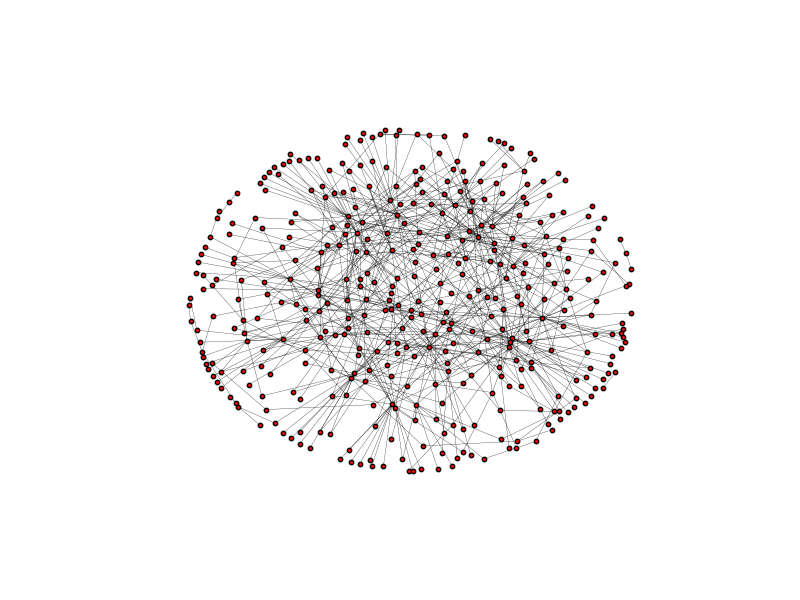
\includegraphics[width=0.49\linewidth]{fig/Results/Exp1/_graph5}\label{fig:exp1SN5}}
    \hfill
    \subfigure[]{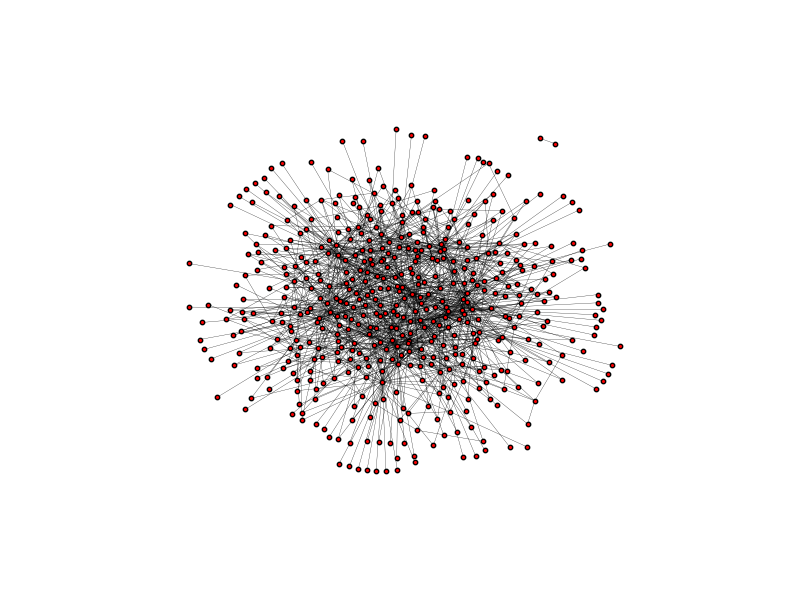
\includegraphics[width=0.49\linewidth]{fig/Results/Exp1/_graph20}\label{fig:exp1SN20}}
    \par \bigskip
    \subfigure[]{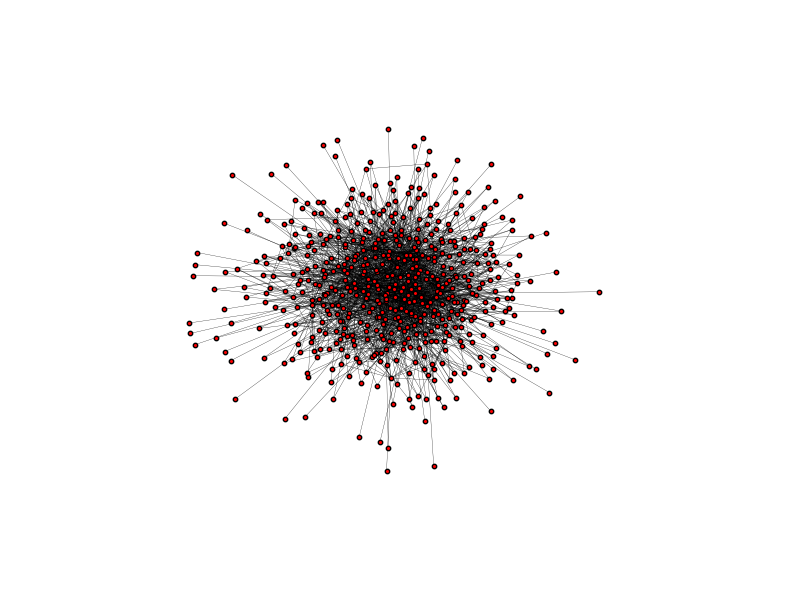
\includegraphics[width=0.49\linewidth]{fig/Results/Exp1/_graph40}\label{fig:exp1SN40}}
    \hfill
    \subfigure[]{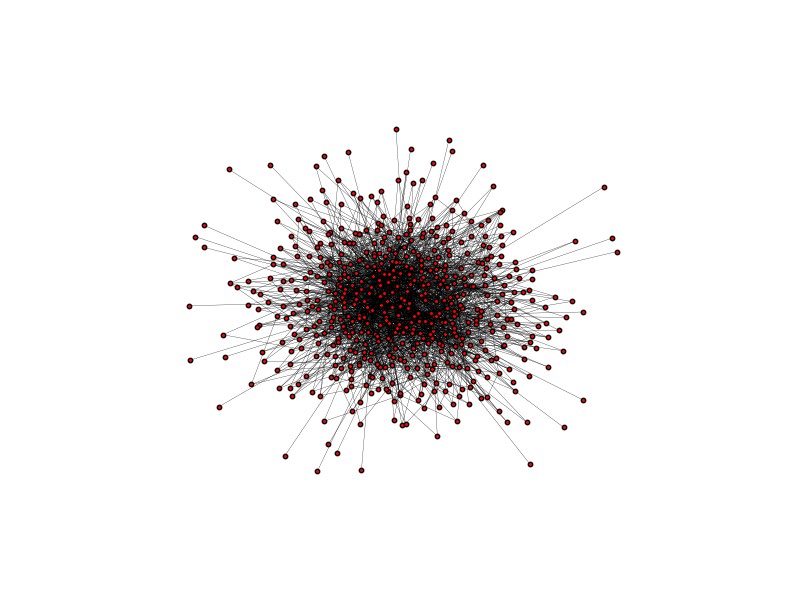
\includegraphics[width=0.49\linewidth]{fig/Results/Exp1/_graph100}\label{fig:exp1SN100}}
    \caption{Snapshots of the social network of experiment 1 at generation 5\subref{fig:exp1SN5}, 20\subref{fig:exp1SN20}, 40\subref{fig:exp1SN40}, and 100\subref{fig:exp1SN100}.}
    \label{fig:exp1.2}
\end{figure}

\clearpage
\subsection{Experiment 2 - Small population}
This experiment was conducted with a population of 100. See Figures~\ref{fig:exp2.0}, \ref{fig:exp2.1}, and \ref{fig:exp2.2} for the Figures related to this experiment. The variance seems to be higher with fewer agents, causing the average fitness and degree to vary more from one generation to another, as seen in Figures~\ref{fig:exp2.0}\subref{fig:Fitness2} and \ref{fig:exp2.0}\subref{fig:Degree2}. The average fitness seems to stabilise at about $0.85$ after generation $30$, which was earlier than in the main experiment. The percentage of successful dialogues reached $90\%$ after only $15$ generations, as seen in Figure~\ref{fig:exp2.1}\subref{fig:succDia2}, and the number of unique highest weighted words reached $1$ after $15$ generations as well, as seen in Figure~\ref{fig:exp2.1}\subref{fig:uniqueWords2}. At generation $5$, the social network consisted of a few agents with two or three edges per agent, as seen in Figure~\ref{fig:exp2.2}\subref{fig:exp2SN5}. Up until generation $40$, the social network became more and more dense for each generation that went by, as seen in Figure~\ref{fig:exp2.2}\subref{fig:exp2SN40}. Between generation $40$ and $100$, there seemed to be little change in the structure of the social network, as seen in Figure~\ref{fig:exp2.2}\subref{fig:exp2SN100}.

\begin{figure}[htbp]
    \centering
    \subfigure[]{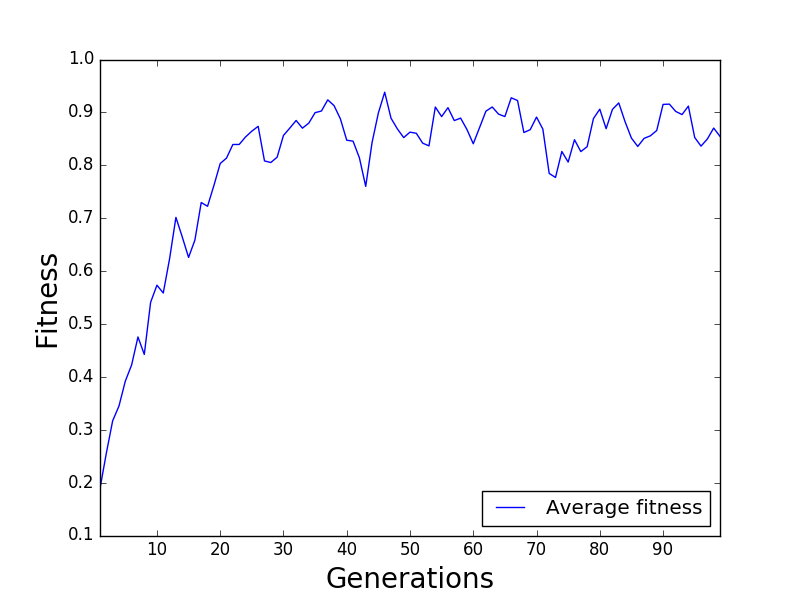
\includegraphics[width=0.49\linewidth]{fig/Results/Exp2/Fitness1}\label{fig:Fitness2}}
    \hfill
    \subfigure[]{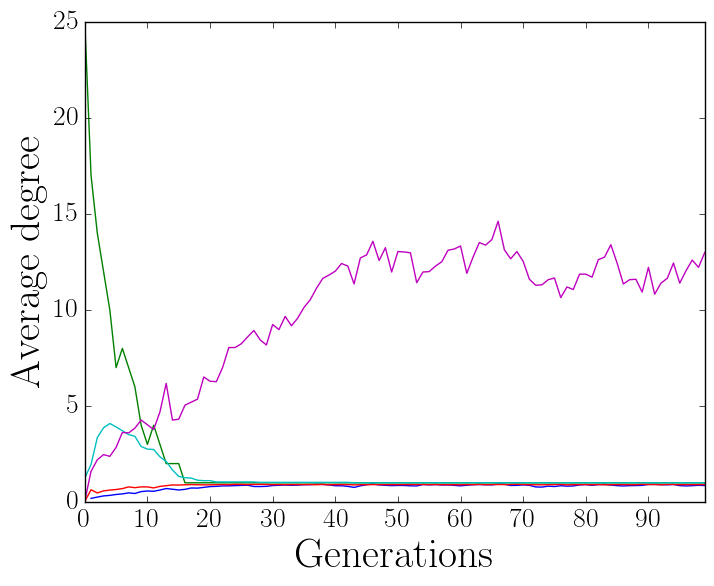
\includegraphics[width=0.49\linewidth]{fig/Results/Exp2/Degree1}\label{fig:Degree2}}
    \caption{Results from experiment 2. \subref{fig:Fitness2}: the average fitness and \subref{fig:Degree2}: the average degree.}
    \label{fig:exp2.0}
\end{figure}
\begin{figure}
    \centering
    \ContinuedFloat
    \subfigure[]{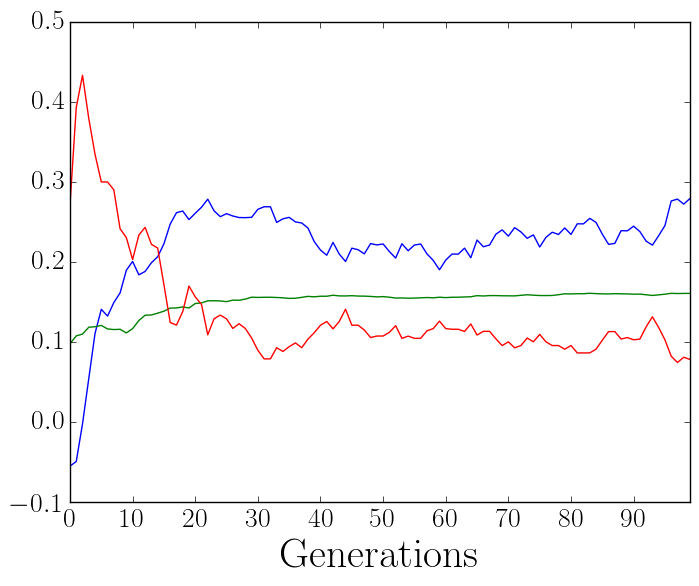
\includegraphics[width=0.49\linewidth]{fig/Results/Exp2/Genes1}\label{fig:exp2Genes}}
    \hfill
    \subfigure[]{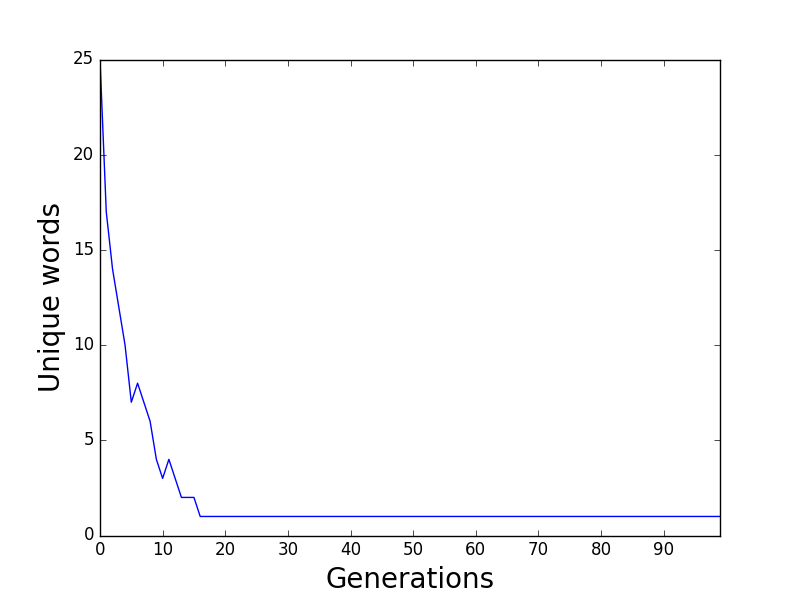
\includegraphics[width=0.49\linewidth]{fig/Results/Exp2/UniqueWords1}\label{fig:uniqueWords2}}
    \par \bigskip
    \subfigure[]{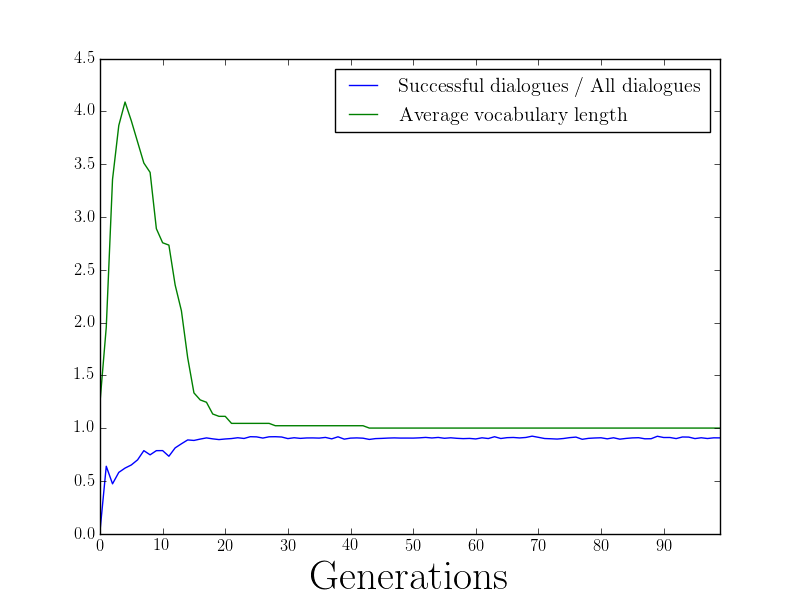
\includegraphics[width=0.49\linewidth]{fig/Results/Exp2/Vocabulary1}\label{fig:Vocabulary2}}
    \hfill
    \subfigure[]{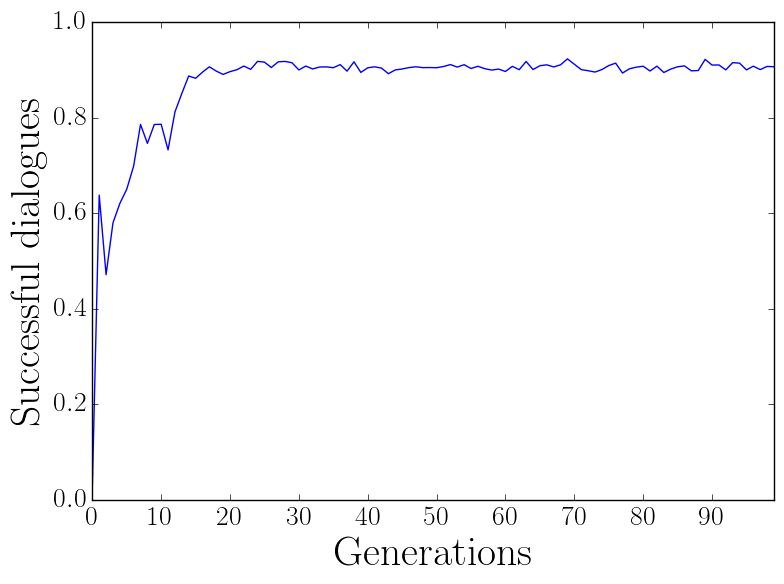
\includegraphics[width=0.49\linewidth]{fig/Results/Exp2/SuccDialogues1}\label{fig:succDia2}}
    \caption{Results from experiment 2. \subref{fig:exp2Genes}: the evolution of the traits from the genome. The three graphs in the figure are the green graph which is the average probability of conducting parent-child dialogues, the blue graph which is the average learning rate, and the  red graph which is the average probability of acting extrovertly. \subref{fig:uniqueWords2}: the number of unique highest ranked words in the population. \subref{fig:Vocabulary2}: average vocabulary size. \subref{fig:succDia2}: successful dialogues divided by total number of dialogues.}
    \label{fig:exp2.1}
\end{figure}
\begin{figure}[htbp]
    \centering
    \subfigure[]{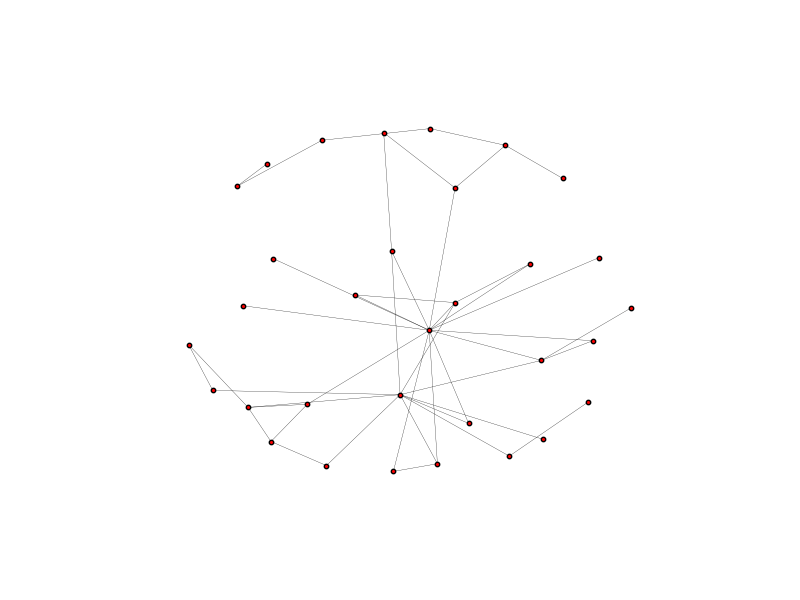
\includegraphics[width=0.49\linewidth]{fig/Results/Exp2/_graph5}\label{fig:exp2SN5}}
    \hfill
    \subfigure[]{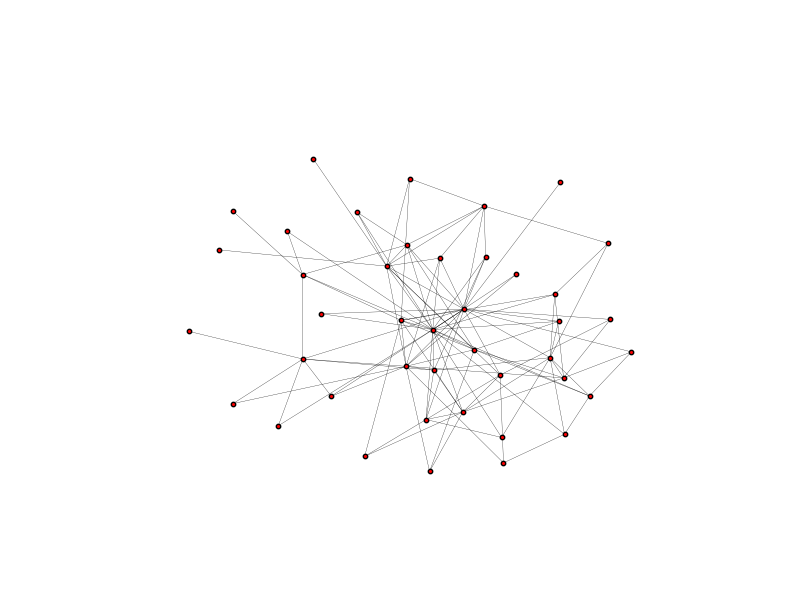
\includegraphics[width=0.49\linewidth]{fig/Results/Exp2/_graph20}\label{fig:exp2SN20}}
    \subfigure[]{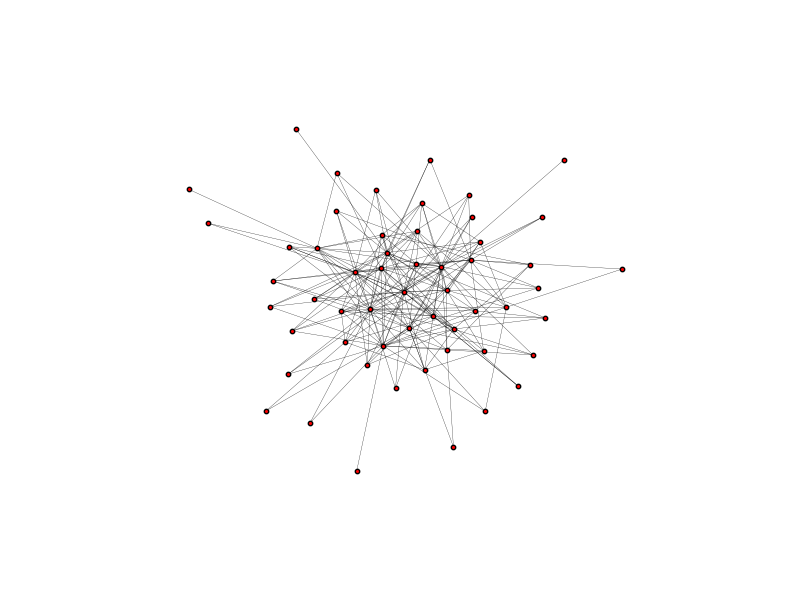
\includegraphics[width=0.49\linewidth]{fig/Results/Exp2/_graph40}\label{fig:exp2SN40}}
    \hfill
    \subfigure[]{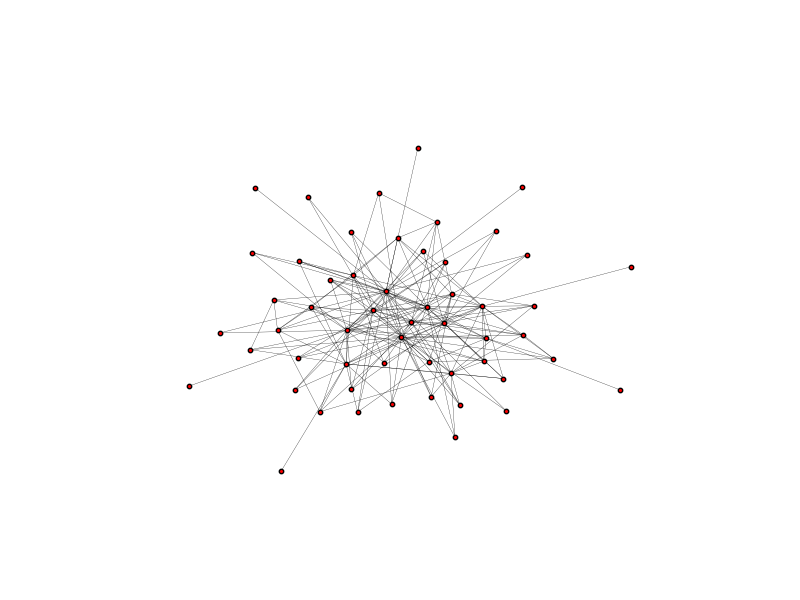
\includegraphics[width=0.49\linewidth]{fig/Results/Exp2/_graph100}\label{fig:exp2SN100}}
    \caption{Snapshots of the social network of experiment 2 at generation 5\subref{fig:exp2SN5}, 20\subref{fig:exp2SN20}, 40\subref{fig:exp2SN40}, and 100\subref{fig:exp2SN100}.}
    \label{fig:exp2.2}
\end{figure}

\clearpage
\subsection{Experiment 3 - Large population}
This experiment was performed with a population of $10000$. See Figure~\ref{fig:exp3.0}, \ref{fig:exp3.0} for the figures related to this experiment. The results show that when there were many agents, they required more time to reach consensus, as seen in Figure~\ref{fig:exp3.1}\subref{fig:uniqueWords3}. In fact, after 100 generations, the agents had not reached an agreement upon one word. This lead to communication more often being unsuccessful, as seen in Figure~\ref{fig:exp3.1}\subref{fig:succDia3}, which again lead to the average fitness and degree being lower than in the results from the main experiment, as seen in Figures~\ref{fig:exp3.0}\subref{fig:Fitness3} and \ref{fig:exp3.0}\subref{fig:Degree3}. The difference in the social network is that the agents were divided into one main group and several other groups of two to three agents for the first generations, as seen in Figure~\ref{fig:exp3.2}.

\begin{figure}[htbp]
    \centering
    \subfigure[]{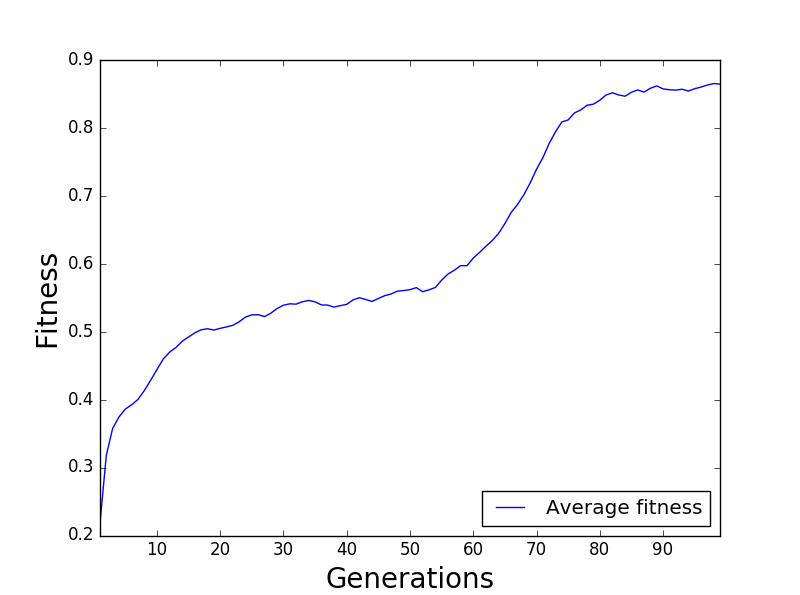
\includegraphics[width=0.49\linewidth]{fig/Results/Exp3/Fitness1}\label{fig:Fitness3}}
    \hfill
    \subfigure[]{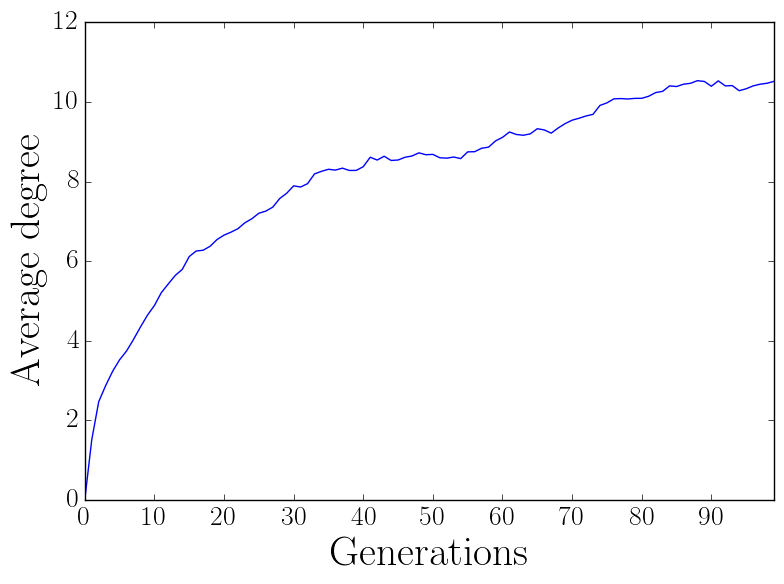
\includegraphics[width=0.49\linewidth]{fig/Results/Exp3/Deg1}\label{fig:Degree3}}
    \caption{Results from experiment 3. \subref{fig:Fitness3}: the average fitness and \subref{fig:Degree3}: the average degree.}
    \label{fig:exp3.0}
\end{figure}
\begin{figure}
    \centering
    \ContinuedFloat
    \subfigure[]{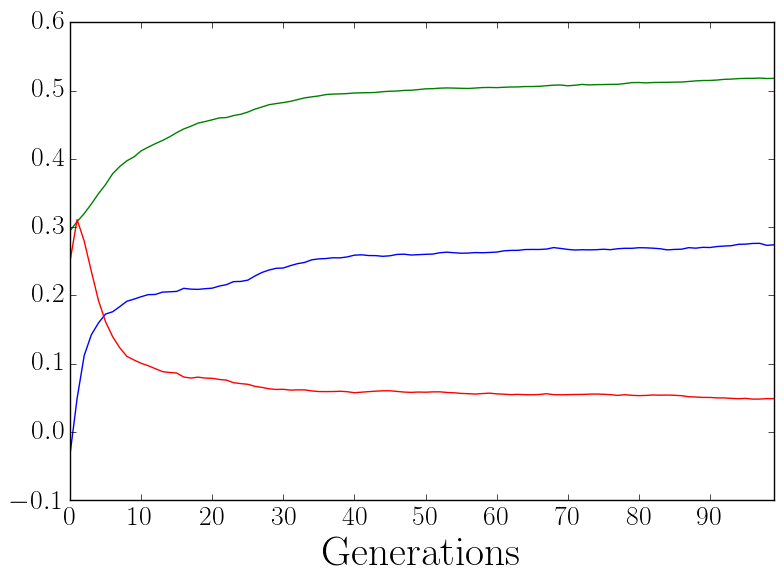
\includegraphics[width=0.49\linewidth]{fig/Results/Exp3/Genes1}\label{fig:exp3Genes}}
    \hfill
    \subfigure[]{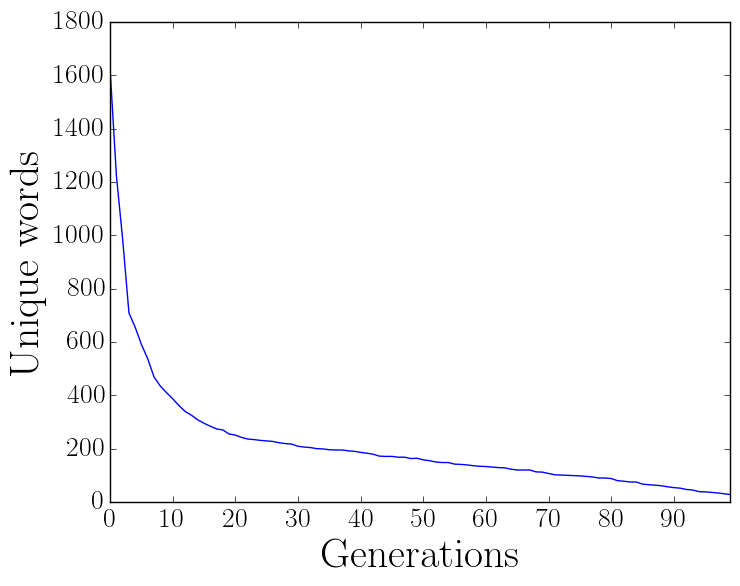
\includegraphics[width=0.49\linewidth]{fig/Results/Exp3/UniqueWords1}\label{fig:uniqueWords3}}
    \par \bigskip
    \subfigure[]{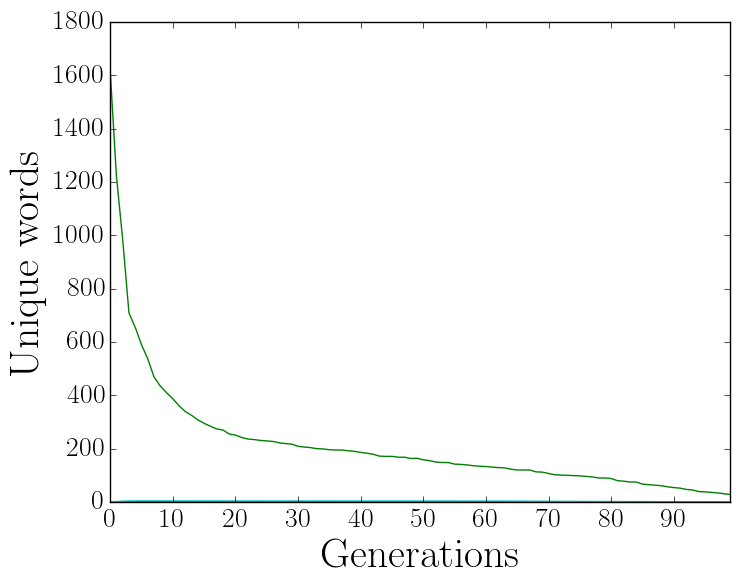
\includegraphics[width=0.49\linewidth]{fig/Results/Exp3/Vocabulary1}\label{fig:Vocabulary3}}
    \hfill
    \subfigure[]{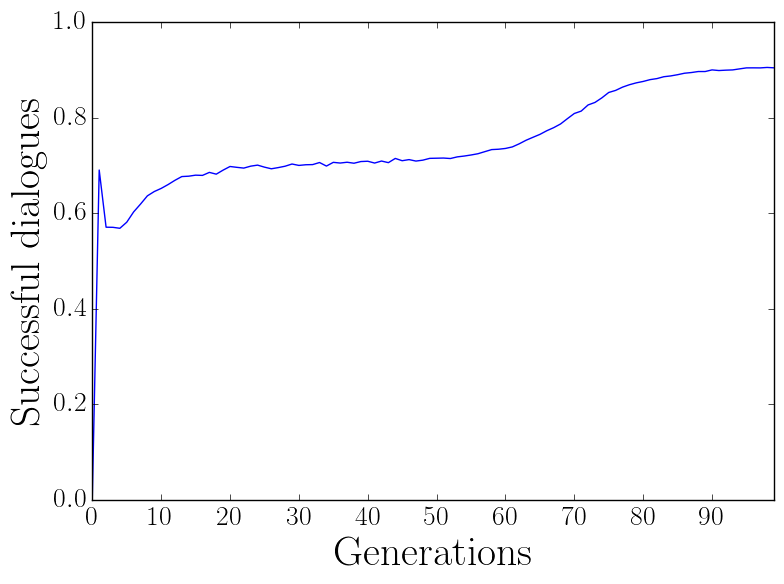
\includegraphics[width=0.49\linewidth]{fig/Results/Exp3/SuccDialogues1}\label{fig:succDia3}}
    \caption{Results from experiment 3. \subref{fig:exp3Genes}: the evolution of the traits from the genome. The three graphs in the figure are the green graph which is the average probability of conducting parent-child dialogues, the blue graph which is the average learning rate, and the  red graph which is the average probability of acting extrovertly. \subref{fig:uniqueWords3}: the number of unique highest ranked words in the population. \subref{fig:Vocabulary3}: average vocabulary size. \subref{fig:succDia3}: successful dialogues divided by total number of dialogues.}
    \label{fig:exp3.1}
\end{figure}
\begin{figure}[htbp]
    \centering
    \subfigure[]{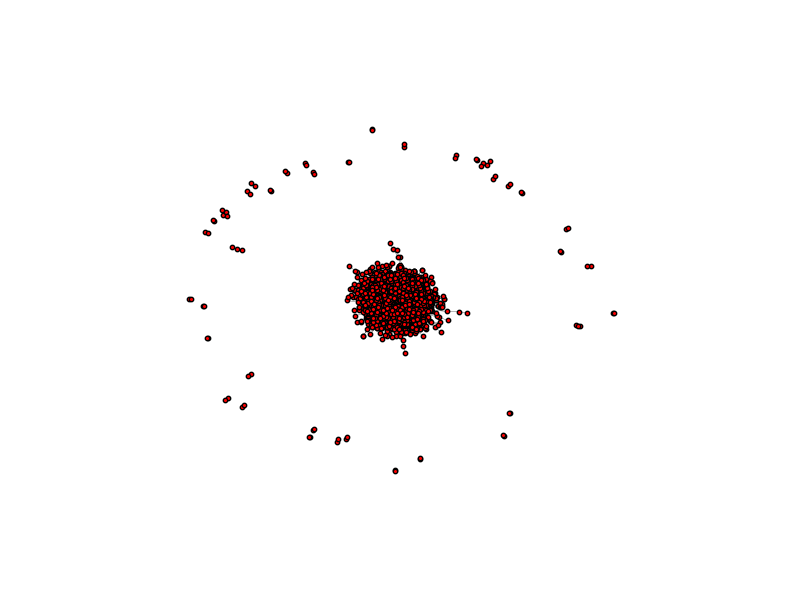
\includegraphics[width=0.49\linewidth]{fig/Results/Exp3/_graph5}\label{fig:exp3SN5}}
    \hfill
    \subfigure[]{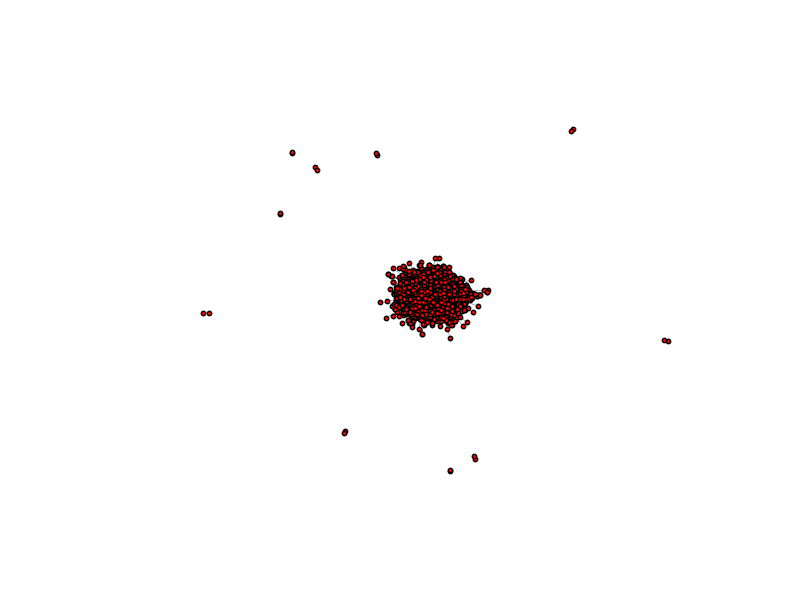
\includegraphics[width=0.49\linewidth]{fig/Results/Exp3/_graph10}\label{fig:exp3SN10}}
    \par \bigskip
    \subfigure[]{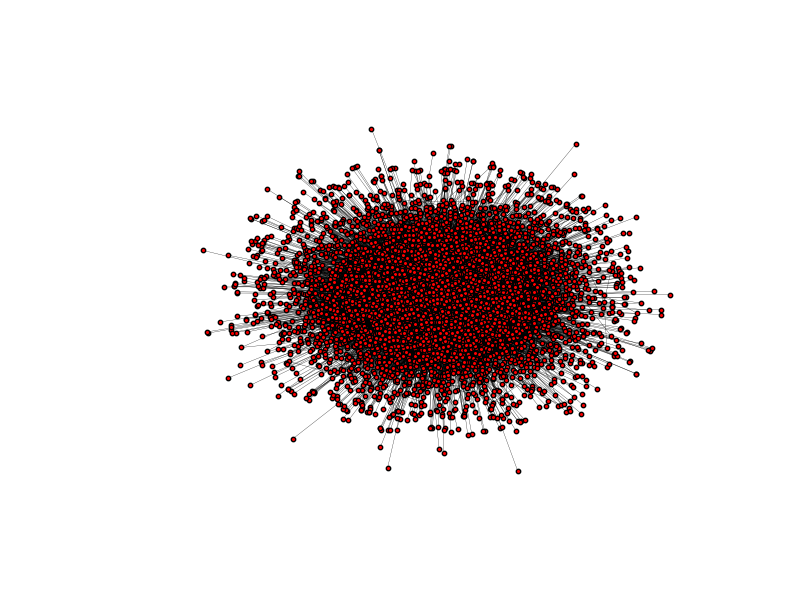
\includegraphics[width=0.49\linewidth]{fig/Results/Exp3/_graph40}\label{fig:exp3SN40}}
    \hfill
    \subfigure[]{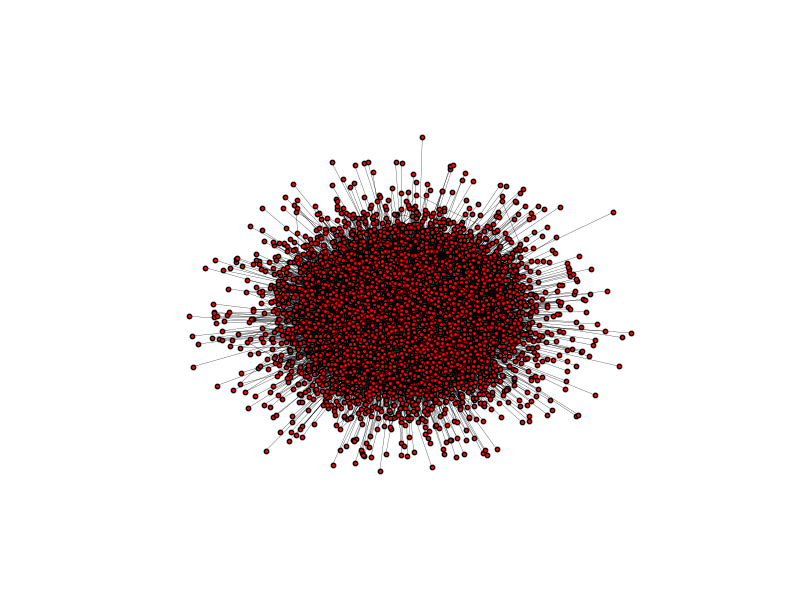
\includegraphics[width=0.49\linewidth]{fig/Results/Exp3/_graph100}\label{fig:exp3SN100}}
    \caption{Snapshots of the social network of experiment 3 at generation 5\subref{fig:exp3SN5}, 10\subref{fig:exp3SN10}, 40\subref{fig:exp3SN40}, and 100\subref{fig:exp3SN100}.}
    \label{fig:exp3.2}
\end{figure}

\clearpage
\subsection{Experiment 4 - Dialogues}
This experiment was conducted with $d = 5$, meaning that each generation conducted five times as many dialogues as in experiment $1$. See Figures~\ref{fig:exp4.0} and \ref{fig:exp4.1} for the graphs related to this experiment. The average degree increased when five times as many dialogues were conducted, as seen in Figure~\ref{fig:exp4.0}\subref{fig:Degree4}. The increase in dialogues ensures that each agent has more and stronger connections leading to a higher average fitness, as seen in Figure~\ref{fig:exp4.0}\subref{fig:Fitness4}. The simulation reached consensus at about the same time as the main experiment, as seen in Figure~\ref{fig:exp4.1}\subref{fig:uniqueWords4}. The probability of acting extrovertly stagnated at about $16\%$, which is almost three times more than experiment 1, as seen in Figure~\ref{fig:exp4.1}\subref{fig:Genes4} The social network evolved similarly as in the main experiment, except that the agents on average had more edges.

\begin{figure}[htbp]
    \centering
    \subfigure[]{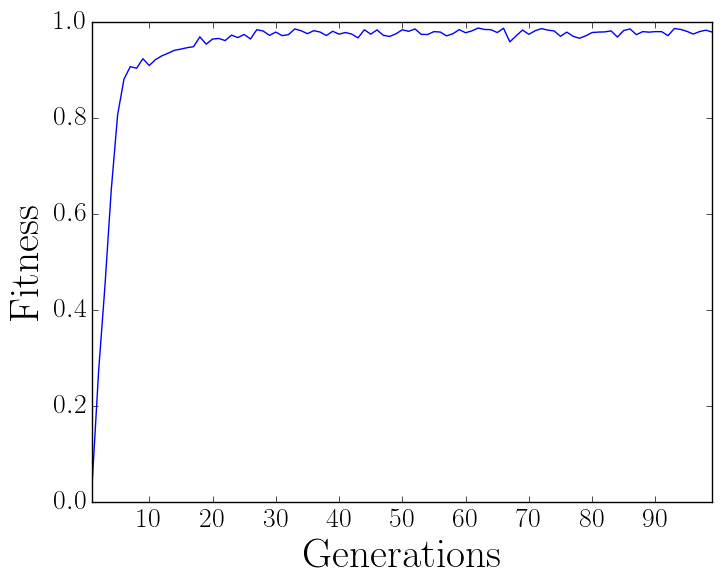
\includegraphics[width=0.49\linewidth]{fig/Results/Exp4/Fitness1}\label{fig:Fitness4}}
    \hfill
    \subfigure[]{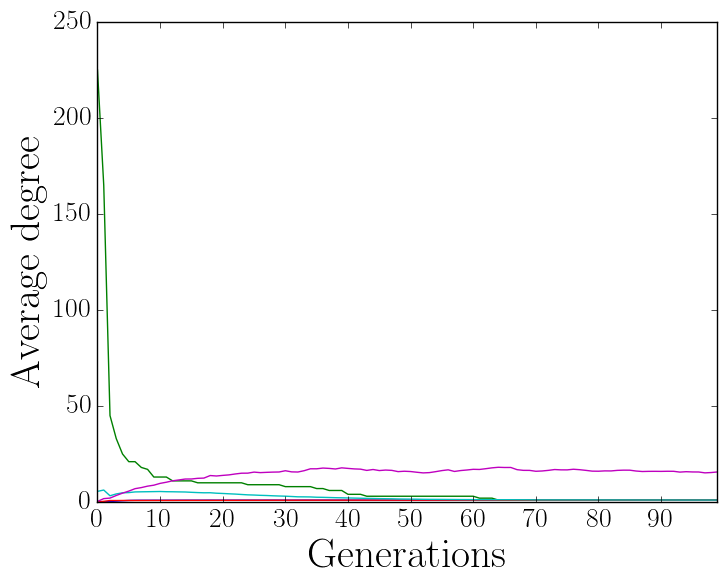
\includegraphics[width=0.49\linewidth]{fig/Results/Exp4/Degree1}\label{fig:Degree4}}
    \caption{Results from experiment 4. \subref{fig:Fitness4}: the average fitness and \subref{fig:Degree4}: the average degree.}
    \label{fig:exp4.0}
\end{figure}
\begin{figure}
    \centering
    \ContinuedFloat
    \subfigure[]{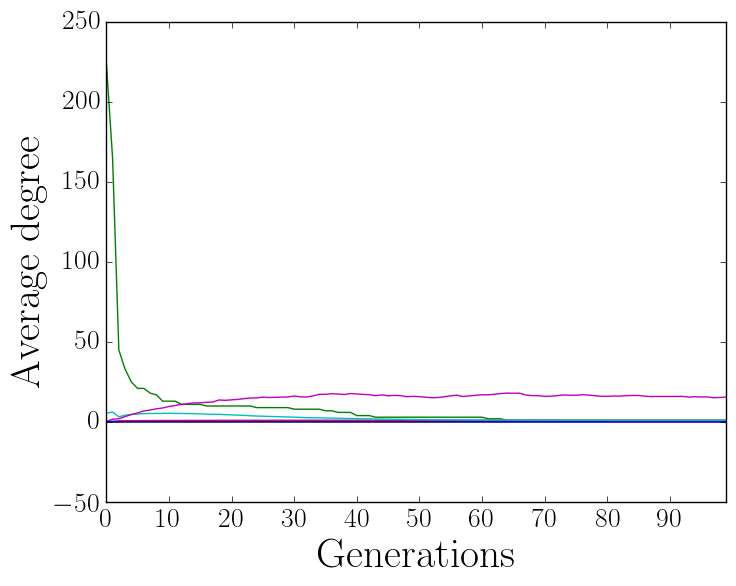
\includegraphics[width=0.49\linewidth]{fig/Results/Exp4/genes1}\label{fig:Genes4}}
    \hfill
    \subfigure[]{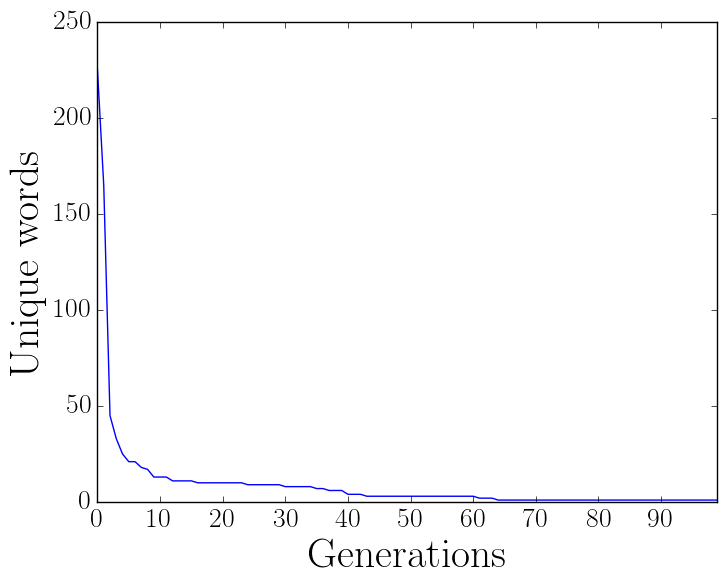
\includegraphics[width=0.49\linewidth]{fig/Results/Exp4/UniqueWords1}\label{fig:uniqueWords4}}
    \par \bigskip
    \subfigure[]{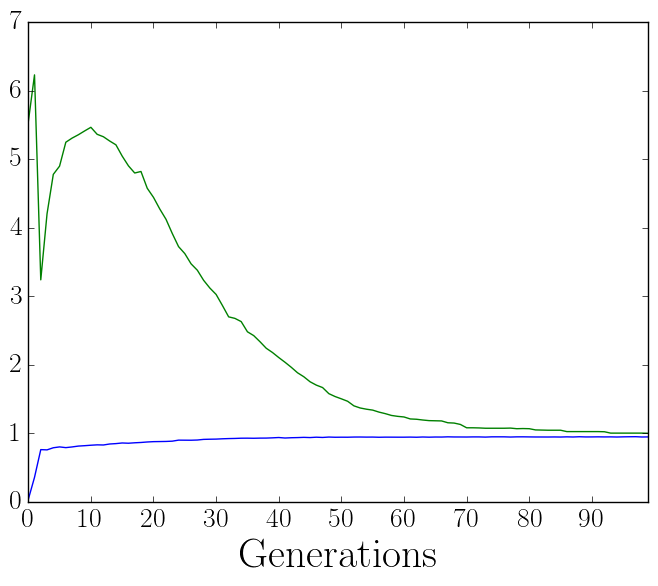
\includegraphics[width=0.49\linewidth]{fig/Results/Exp4/Vocabulary1}\label{fig:Vocabulary4}}
    \hfill
    \subfigure[]{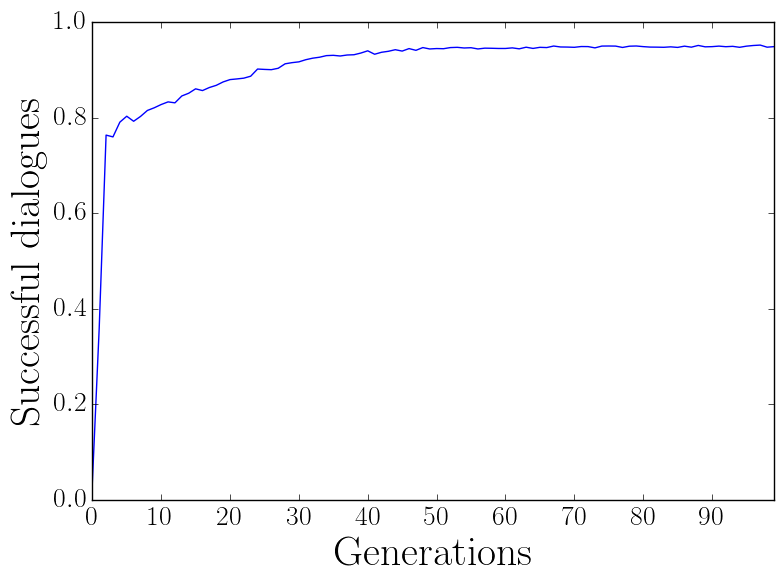
\includegraphics[width=0.49\linewidth]{fig/Results/Exp4/SuccDialogues1}\label{fig:succDia4}}
    \caption{Results from experiment 4. \subref{fig:Genes4}: the evolution of the traits from the genome. The three graphs in the figure are the green graph which is the average probability of conducting parent-child dialogues, the blue graph which is the average learning rate, and the  red graph which is the average probability of acting extrovertly. \subref{fig:uniqueWords4}: the number of unique highest ranked words in the population. \subref{fig:Vocabulary4}: average vocabulary size. \subref{fig:succDia4}: successful dialogues divided by total number of dialogues.}
    \label{fig:exp4.1}
\end{figure}

\clearpage
\subsection{Experiment 5 - Less Parent-child dialogues}
This experiment was conducted with the constant $\delta = 1$. $\delta$ is related to the probability of a child having its first dialogues with its parents. See figures~\ref{fig:exp5.0} and \ref{fig:exp5.1} for the figures related to this experiment. The simulation was ran for $150$ generations, e.g. $g = 150$, because it did not reach consensus after $100$ generations, and knowing how this simulation evolved up until consensus might be interesting. The average fitness increased slowly during the entire simulation, as seen in Figure~\ref{fig:exp5.0}\subref{fig:Fitness5}. The average degree reached four at generation $70$, and during the next $80$ generations the average only increased by $0.5$, as seen in Figure~\ref{fig:exp5.0}\subref{fig:Degree5}. The percentage of successful dialogues quickly reached $60\%$, and slowly increased during the entire simulation ending at $93\%$, as seen in Figure~\ref{fig:exp5.1}\subref{fig:succDia5}. The average vocabulary size increased during the first $25$ generations, and then decreased and ended at $1.04$, as seen in Figure~\ref{fig:exp5.1}\subref{fig:Vocabulary5}. The simulation reached consensus at generation $127$, as seen in Figure~\ref{fig:exp5.1}\subref{fig:uniqueWords5}.

\begin{figure}[htbp]
    \centering
    \subfigure[]{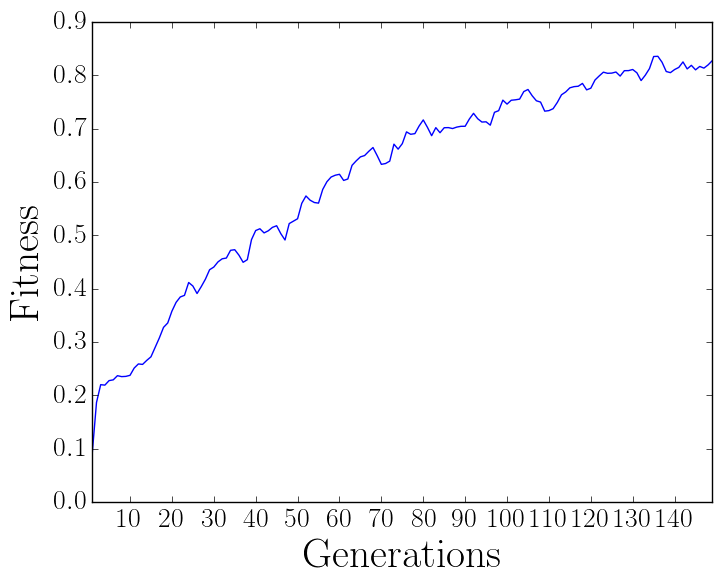
\includegraphics[width=0.49\linewidth]{fig/Results/Exp5/Fitness1}\label{fig:Fitness5}}
    \hfill
    \subfigure[]{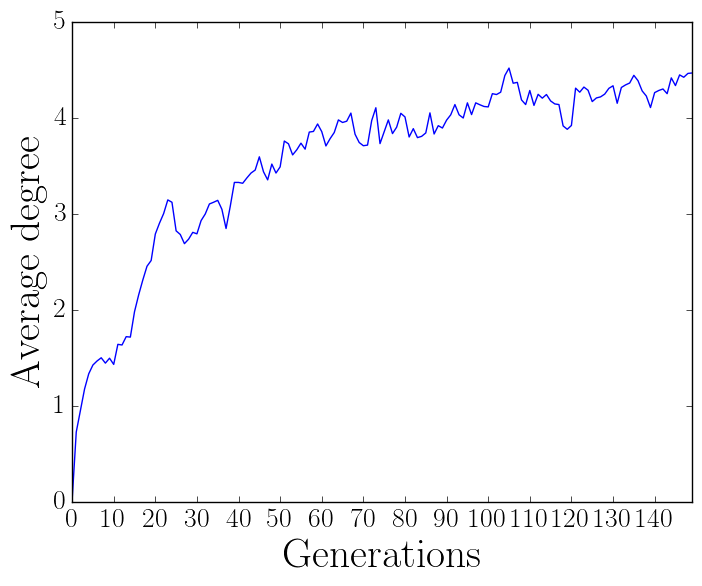
\includegraphics[width=0.49\linewidth]{fig/Results/Exp5/Degree1}\label{fig:Degree5}}
    \caption{Results from experiment 5. \subref{fig:Fitness5}: the average fitness and \subref{fig:Degree5}: the average degree.}
    \label{fig:exp5.0}
\end{figure}
\begin{figure}
    \centering
    \ContinuedFloat
    \subfigure[]{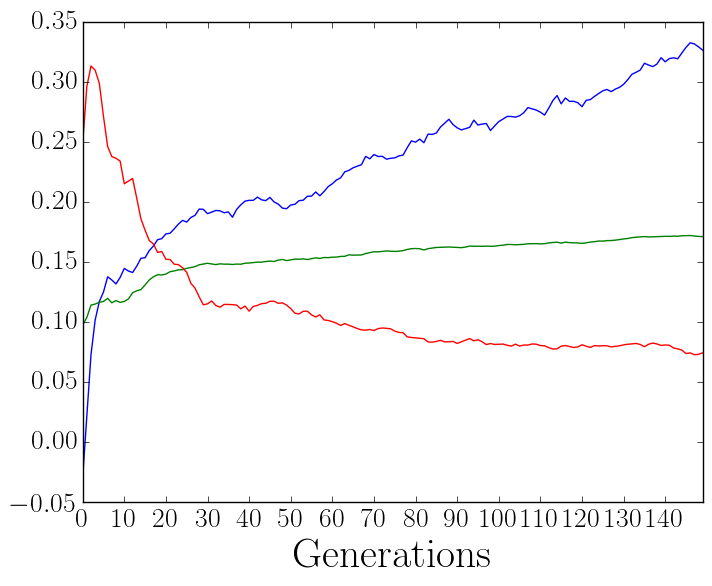
\includegraphics[width=0.49\linewidth]{fig/Results/Exp5/Genes1}\label{fig:Genes5}}
    \hfill
    \subfigure[]{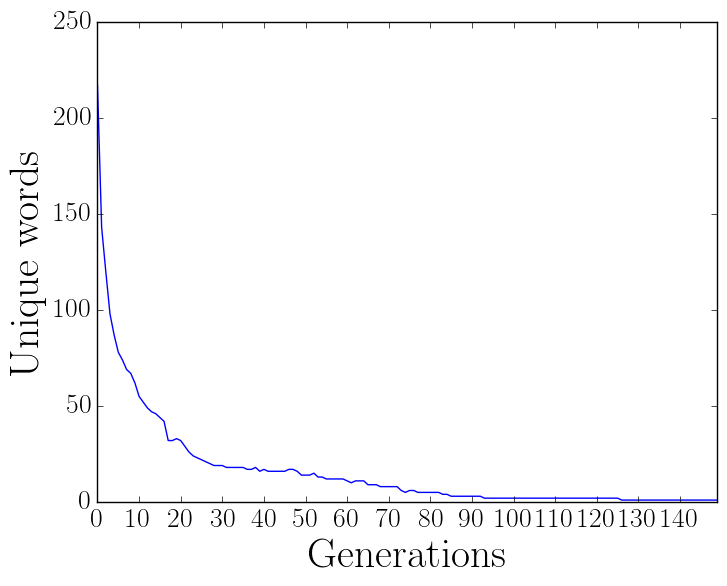
\includegraphics[width=0.49\linewidth]{fig/Results/Exp5/UniqueWords1}\label{fig:uniqueWords5}}
    \par \bigskip
    \subfigure[]{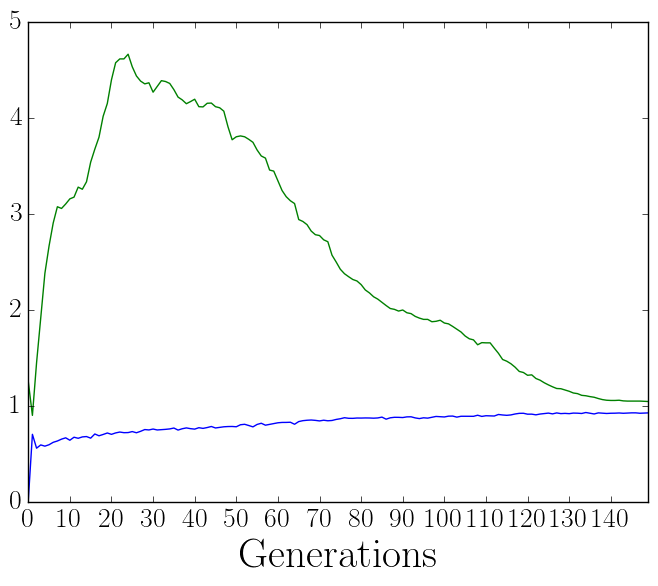
\includegraphics[width=0.49\linewidth]{fig/Results/Exp5/Vocabulary1}\label{fig:Vocabulary5}}
    \hfill
    \subfigure[]{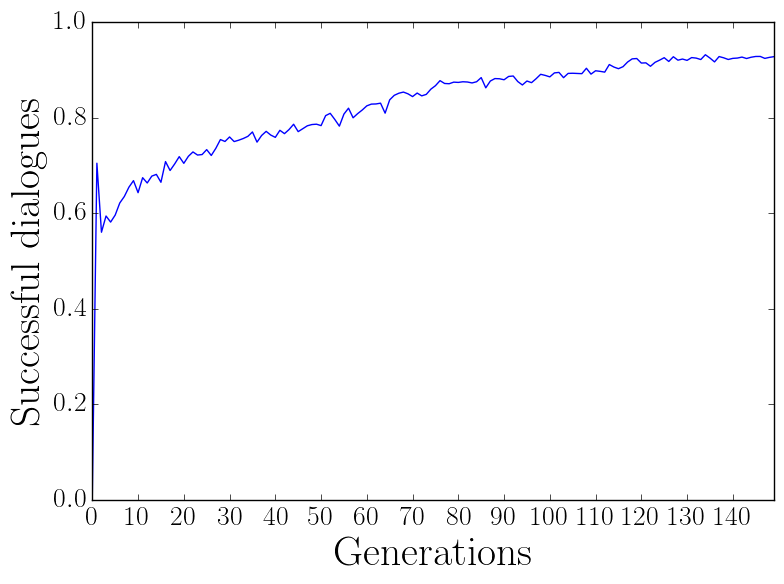
\includegraphics[width=0.49\linewidth]{fig/Results/Exp5/SuccDialogues1}\label{fig:succDia5}}
    \caption{Results from experiment 5. \subref{fig:Genes5}: the evolution of the traits from the genome. The three graphs in the figure are the green graph which is the average probability of conducting parent-child dialogues, the blue graph which is the average learning rate, and the  red graph which is the average probability of acting extrovertly. \subref{fig:uniqueWords5}: the number of unique highest ranked words in the population. \subref{fig:Vocabulary5}: average vocabulary size. \subref{fig:succDia5}: successful dialogues divided by total number of dialogues.}
    \label{fig:exp5.1}
\end{figure}

\clearpage
\subsection{Experiment 6 - Turnover}
%
Experiment 6 was performed in two parts, part 6a with $k = 0.95$ and $n = 0.7$, compared to $k = 0.9$ and $n = 0.5$ in the other experiments. This means that a larger portion (n) of the population was chosen for survival and from a larger selection pool (K). Figures~\ref{fig:exp6.0} and \ref{fig:exp6.1} show the results of experiment 6. This simulation was run for $150$ generations because the population was far away from reaching consensus after $100$ generations. The figures that display the genes and the evolution of the social network have not been included because they were similar to the ones from the main experiment. Both the average fitness and degree stabilised after about $75$ generations, as can be seen in the Figures~\ref{fig:Fitness6} and \ref{fig:Degree6}. The average degree stabilised at $11$ and the average fitness at $0.88$. The number of unique words decreased a lot during the first $20$ generations, as can be seen in Figure~\ref{fig:uniqueWords6}. The simulation did not reach consensus. It reached two unique words at generation $125$, and also ended with two unique words after all $150$ generations.   

Experiment 6b was conducted with $k = 0.95$ and $n = 0.85$ which allowed a larger portion of the fittest agents to survive each generation, giving the simulation a lower selection pressure. Experiment 6b was conducted in order to see what happened when the selection pressure was lower than in experiment 6b. Figure ~\ref{fig:uniqueWords6} compares how experiment 6a and 6b evolved towards consensus. Experiment 6b was ran for $200$ generations in order for it to reach consensus. Consensus was reached at generation $178$. At generation $125$, when experiment 6a had reached two words, this simulation had six unique words. 

\begin{figure}[htbp]
    \centering
    \subfigure[]{\includegraphics[width=0.49\linewidth]{fig/Results/Exp6/Fitness1}\label{fig:Fitness6}}
    \hfill
    \subfigure[]{\includegraphics[width=0.49\linewidth]{fig/Results/Exp6/Degree1}\label{fig:Degree6}}
    \caption{Results from experiment 6. \subref{fig:Fitness6}: the average fitness and \subref{fig:Degree6}: the average degree.}
    \label{fig:exp6.0}
\end{figure}
\begin{figure}
    \centering
    \ContinuedFloat
    \subfigure[]{\includegraphics[width=0.49\linewidth]{fig/Results/Exp6/Vocabulary1}\label{fig:Vocabulary6}}
    \hfill
    \subfigure[]{\includegraphics[width=0.49\linewidth]{fig/Results/Exp6/SuccDialogues1}\label{fig:succDia6}}
    \par \bigskip
    \subfigure[]{\includegraphics[width=0.6\linewidth]{fig/Results/Exp6/UniqueWordsAB}\label{fig:uniqueWords6}}
    \caption{Results from experiment 6. \subref{fig:Vocabulary6}: average vocabulary size of experiment 6a. \subref{fig:succDia6}: successful dialogues divided by total number of dialogues of experiment 6a. \subref{fig:uniqueWords6}: the number of unique highest ranked words in the population of experiment 6 a and b.}
    \label{fig:exp6.1}
\end{figure}

\clearpage
\subsection{Experiment 7 - making up new words}
Experiment 7 was conducted in two parts, both with an added probability for agents to invent a new word even though they had at least one word in their vocabulary. See Figures~\ref{fig:exp7.0} and \ref{fig:exp7.1} for the results from the two parts of the experiment.

Experiment 7a was performed with the probability of inventing a new word set to $25\%$. The average fitness stabilised at $0.37$, and the average degree stabilised at about $6.5$, as seen in Figures~\ref{fig:Fitness7} and \ref{fig:Degree7}. Both of these values were considerably lower than in experiment $1$. Figures~\ref{fig:Vocabulary7} and \ref{fig:succDia7} show that average vocabulary size was $6$ and the percentage of successful dialogues quickly reached $0.5$ but it did not slowly increase like in the previous experiments. The number of unique highest ranked words evolved similarly to experiment $1$, as seen in Figure~\ref{fig:uniqueWords7}. The population reached consensus at generation $68$, only six generations experiment $1$. 

Experiment 7b was performed with the probability of inventing a word increased to $45\%$. See figure~\ref{fig:uniqueWords7} for the figure related to this experiment. The other graphs have not been included because the purpose of this experiment was to see how the evolution towards consensus changed with a higher probability of inventing a word. The number of unique words quickly dropped to about five, but from five it struggled to actually reach consensus. Experiment 7b reached consensus at generation $73$, but that only lasted a few generations. For the remainder of the simulation, the number of unique words varied from one to four. 

\begin{figure}[htbp]
    \centering
    \subfigure[]{\includegraphics[width=0.49\linewidth]{fig/Results/Exp7/Fitness1}\label{fig:Fitness7}}
    \hfill
    \subfigure[]{\includegraphics[width=0.49\linewidth]{fig/Results/Exp7/Degree1}\label{fig:Degree7}}
    \caption{Graphs from experiment 7.}
    \label{fig:exp7.0}
\end{figure}
\begin{figure}
    \centering
    \ContinuedFloat
    \subfigure[]{\includegraphics[width=0.49\linewidth]{fig/Results/Exp7/Genes1}\label{fig:Genes7}}
    \hfill
    \subfigure[]{\includegraphics[width=0.49\linewidth]{fig/Results/Exp7/Vocabulary1}\label{fig:Vocabulary7}}
    \par \bigskip
    \subfigure[]{\includegraphics[width=0.49\linewidth]{fig/Results/Exp7/SuccDialogues1}\label{fig:succDia7}}
    \hfill
    \subfigure[]{\includegraphics[width=0.49\linewidth]{fig/Results/Exp7/UniqueWordsAB}\label{fig:uniqueWords7}}
    \caption{Results from experiment 7. \subref{fig:Genes7}: the evolution of the traits from the genome. The three graphs in the figure are the green graph which is the average probability of conducting parent-child dialogues, the blue graph which is the average learning rate, and the  red graph which is the average probability of acting extrovertly. \subref{fig:Vocabulary6}: average vocabulary size of experiment 7a. \subref{fig:succDia6}: successful dialogues divided by total number of dialogues of experiment 7a. \subref{fig:uniqueWords6}: the number of unique highest ranked words in the population of experiment 7a and b.}
    \label{fig:exp7.1}
\end{figure}
\acresetall
%%=========================================
\chapter{Discussion}
In the main experiment, the evolution was in favour of agents that acted extrovert during the first generation, because most dialogues were unsuccessful, see figure \ref{fig:Genes1} for the evolution of the traits. As the number of unique words decreased, introvert dialogues became more likely to be successful, and a successful dialogue increased the involved agents' fitness. An extrovert agent had many edges, which increased its fitness. On the other hand, those edges had a lower average weight than an agent with fewer edges. A low average weight would decrease the agent's fitness. So there was a trade-off between acting introvertly and having fewer edges with high weights, and acting extrovertly and having more edges with lower weights. The population evolved towards favouring introvert characteristics. Agents also evolved towards higher learning rate, most likely because a high learning rate made the language easier to learn. When the population had almost reached consensus, and the average vocabulary length was close to $1.0$, the average learning rate stopped increasing. This might have happened because the newborns were only taught one word which made the learning unimportant. 

The first ten generations, the number of unique highest ranked words dropped. The agents that got edges of a certain weight survived the first generations. Those agents had a high fitness and were probable to be chosen as parents several times during the parent selection phase. The agents that got selected as parents several times and had a high probability of speaking to their children acquired more edges with strong weights, which increased their fitness and likelihood of surviving to the next generation. This cycle kept a select few agents alive for the first generations, allowing them to spread their language to many others. This is how the number of unique words dropped quickly during the first generations of the simulation. 

The average vocabulary length increased during the first seven generations because most did not have one word with a much higher weight than the others, see figure \ref{fig:VocComp}. Also, most children were taught at least two words, usually more, during the first generations. Most of the words they were taught got a very low weight and less words were passed on as the generations passed by. In order to gain edges during the first generation, the agents acted extroverted, which lead to them learning or teaching new words which made the average vocabulary size increase. When a few words in the vocabularies had gotten a significantly higher weight than the others, those words were the only words that the newborn agents learned. The process where newborns only picked up the most successful words of their parents quickly reduced the number of unique words and the average vocabulary length. After the first ten generations, the evolution towards consensus continued slowly. 
 
The social network became denser as the population evolved, up until generation $40$ which was when the average degree of the agents stabilised. Even though the agents mainly acted introvertly, the social network was not divided into groups, like in Lekvam’s experiment \citep[Section 5.1]{lekvam2014co}. The reason why this is the case probably was because every agent could contact any other agent when it acted extrovertly. This meant that the entire population existed without any physical distance from one another. A community of individuals living so close to each other might evolve a social network similar to the one from this simulation. The network consisted of several circular layers, where the innermost layer had agents with the most edges, and the outer layer had agents with the fewest edges.

Experiment 2 reached consensus after fewer generations than experiment 1, see figure \ref{fig:hrwComp}. This happened because there were fewer words to begin with and fewer agents to teach one word to. One agent with a high probability was more likely to become a parent in a small population, which lead to more newborns that learned the same word from an earlier generation. The tendencies concerning how the language evolved were similar, only that it all happened faster with higher variance. Especially the average degree and fitness had big variations from one generation to another compared to experiment 1. See figure \ref{fig:fitComp} for the fitness and figure \ref{fig:degreeComp} for the degree. This is natural considering that there were randomness involved in the form of choosing the agents involved in dialogues, and making children. When fewer dialogues and fewer children were made per generation, the variance increase.

Experiment 3 should have less variance and have required more generations to reach consensus than experiment 1 if this reasoning was correct, and it had less variance and reached consensus later. The evolution began similarly the two previous experiments, where the population's average degree, fitness and unique words evolved quickly. See figure \ref{fig:fitComp} for the fitness, figure \ref{fig:degreeComp} for the degree, and figure \ref{fig:hrwComp} for the unique highest words. The population stabilised on a high number of unique words and a fitness of $0.5$. At generation $60$, the parents taught their children a few words and the average vocabulary length started falling, and the average fitness increased, see figure \ref{fig:VocComp}. This is exactly what happened in experiment 1, only that the population in experiment 3 required more time to reach a state where the words had a significantly higher weight, because of the population’s size. 

The social network had small groups of two agents for many generations. Those small groups eventually died out or joined the main group because the small groups were unable to get a big enough fitness on their own. This happened more slowly because the newborns in the main group learned many different words from their parents, giving the agents in the main group a lower average fitness than the main group in the two previous experiments.

The number of dialogues per generation was quintupled in experiment 4, and it would be natural to assume that it would allow the population to reach consensus faster than in the main experiment, but it did not, see figure \ref{fig:hrwComp}. It did, however, provide the agents with a higher average fitness because the average weight increased a lot due to the high number of introvert dialogues, see figure \ref{fig:fitComp}. The average degree decreased after the second generation because the parents taught their newborn agents fewer words than what they had in their own vocabularies, see figure \ref{fig:degreeComp}. However, the average quickly increased again, because the newborns shared their learned words through extrovert conversations. The number of extrovert conversations per agent per generation was naturally higher in this simulation. That lead to more newborn agents dying since their parents had a very high fitness. The parents' fitness was high because they had conducted so many dialogues during their lifetime that they had several highly weighted connections. This simulation required the same number of generations to reach consensus as experiment 1, which indicates that the number of dialogues had little effect on reaching consensus. This result lead to the conclusion that the dialogues had a small impact on the agents' vocabulary. The only other method for a newborn to learn a language in this model was through initial conversations with its parents, and this experiment indicate that parent-child dialogues might be important for this model to reach consensus.  

The next experiment tested the hypothesis that on the \textit{ontogenetic} time scale, which concerns how an individual learns language (\ref{EvoltionaryForces}), the most important factor is being taught the a select few languages from an early age. In this model and in reality, the best method for being taught the same languages consistently is through several dialogues with the same persons, usually ones parents. This was tested through the probability of parents speaking to their newborn being set to three times less than in the main experiment. If the hypothesis was to be true, this experiment should have required more generations than the main experiment to reach consensus. Throughout the experiments performed thus far, when the average vocabulary length started decreasing, it seemed to be an indicator of that the population was approaching consensus. In experiment 1, the average vocabulary size started decreasing at generation eight, but in this experiment, the average vocabulary size started decreasing at generation $25$, see figure \ref{fig:VocComp}. Experiment 1 had reached consensus at generation $61$, while this experiment reached consensus at generation $127$, see figure \ref{fig:hrwComp}. This result supports the hypothesis that this computational model's most important factor for reaching consensus is the parents speaking to their children. This also indicates that the first dialogues are essential for the newborns language in this computational model. The language of the children in this computational model is defined through its first dialogues, and after that it is very hard to change primary language, just like humans who tends to struggle when attempting to learn a language at an adult age. 

The average degree was significantly lower than in experiment 1 because a lot of newborns did not get the initial dialogues with their parents, see figure \ref{fig:degreeComp}. The parent-child dialogues were reduced but the experiment had the same number of dialogues, and therefore the same number of extrovert dialogues. This indicates that the average degree should be roughly $1/3$ of the main experiment. The main experiment stabilised on an average degree of about $10$, and this experiment stabilised on an average of about $4$, which is $2.5$ times as few edges as the main experiment.

The social network in this experiment evolved through a few agents that had a much higher fitness and a much higher probability of speaking to their children than the other agents in the population had. Those parents created the fan-like shapes, which was visible at generation $5$ and $10$, see figures \ref{exp5SN5} and \ref{exp5SN10}. At generation $100$, the social network had evolved into a network similar to the network at generation $5$ from experiment 1. See figure \ref{fig:SNComparison} for comparison of the two social networks. The network did not change during the last $50$ generations of the simulation.

\begin{figure}
    \centering
    \subfigure[Experiment 1 at generation 5]{\includegraphics[width=0.49\linewidth]{fig/Results/Exp1/_graph5}}
    \hfill
    \subfigure[Experiment 5 at generation 100]{\includegraphics[width=0.49\linewidth]{fig/Results/Exp5/_graph100}}
    \caption{Comparison of the social network at generation 5 of experiment 1 and generation 100 of experiment 5}
    \label{fig:SNComparison}
\end{figure}

The fact that the social network in this simulation was much less dense indicate that the connections gotten from the initial dialogues were important when it comes to acquiring other connections than an agents parents. This probably is because the probability of becoming a speaker is related to an agents' fitness. An Agent without connections have a fitness of zero, making it unlikely that it would become a speaker. In this experiment, many newborns did not have dialogues with their parents, which lead them to be unlikely to be chosen as speakers, which again lead to the social network being less dense compared to experiment 1. See figure \ref{SNcomp15} for a comparison of the social network of experiment 1 and 5 at generation 100. All features that were affected by the language in this experiment evolved similarly to the main experiment, only significantly slower, which indicates that parents speaking to their children had a big effect on the evolution towards consensus.

\begin{figure}
    \centering
    \subfigure[Social network at generation 100 for experiment 1.]{\includegraphics[width=0.49\linewidth]{fig/Results/Exp1/_graph100}}
    \hfill
    \subfigure[Social network at generation 100 for experiment 5.]{\includegraphics[width=0.49\linewidth]{fig/Results/Exp5/_graph100}}
    \caption{Comparison of the social network of experiment 1 and 5 at generation 100.}
    \label{SNcomp15}
\end{figure}

If the number of newborns being made per generation were less, one could expect to see similar results as the previous experiment because, with fewer newborns per generation, fewer newborns would conduct initial dialogues with their parents. Experiment 6 tested this through increasing the $k$ and $n$ values. The results show that the population struggled to reach consensus, in fact, the population did not reach consensus within the $150$ generations the simulation was ran, see figure \ref{fig:hrwComp}. The result indicates that it is not only important to have many newborns being taught a consistent language in the early years, it is also important that a certain number of newborns are made each generation to allow the evolution to move forward. 

When a larger portion of the population survived each generation, the selection pressure on the population was lessened. When the selection pressure was lessened, the evolutionary forces at the \textit{phylogenetic} and \textit{glossogenetic} had less of an impact, see section \ref{EvoltionaryForces} for a description of the evolutionary forces. The second experiment performed with varying turnover had an even smaller selection pressure, which lead to the language evolving even slower, see figure \ref{fig:hrwComp}. These results indicate that when the selection pressure on a species is small enough it does not need to evolve in order to survive, and then the species will evolve very slowly. In this computational model, when the selection pressure was high enough, the population reached consensus, but when the selection pressure was lessened the evolution towards consensus slowed down. This indicates that the Baldwin effect affects the \textit{phylogenetic} and \textit{glossogenetic} forces of language evolution. 

The average fitness and degree was higher when a larger part of the population survives to the next generation. See figure \ref{fig:fitComp} for the fitness and figure \ref{fig:degreeComp} for the degree. The agents who survive generally are among the fittest of the current population, and so when a larger portion of the agents with a high fitness survive, the average fitness becomes higher. The average degree is directly related to the fitness function, so it is natural that it is higher as well. 

When the agents could make up new words with a probability of $0.25$, one would expect the percentage of successful dialogues to be less and average vocabulary size to be more than in the main experiment. One might also expect that the population would have required more generations to reach consensus when a lot more utterances existed. The average fitness, degree, and percentage of successful dialogues were lower than in the main experiment, and the average vocabulary size was a lot higher. See figure \ref{fig:VocComp} for the vocabulary, figure \ref{fig:fitComp} for the fitness, figure \ref{fig:degreeComp} for the degree and figure \ref{fig:DialogueComp} for the rate of successful dialogues. This did, however, not significantly affect the evolution towards consensus, see figure \ref{fig:hrwComp}. 

\begin{figure}
    \centering
    \includegraphics[width=0.7\linewidth]{fig/Discussion/FitnessComparison}
    \caption{Comparing the fitness per generation for experiment $1$, $2$, $3$, $4$, $6$, $6.1$, and $7.1$.}
    \label{fig:fitComp}
\end{figure}
\begin{figure}
    \centering
    \includegraphics[width=0.7\linewidth]{fig/Discussion/DegreeComparison}
    \caption{Comparing the number of unique highest ranked words per generation for experiment $1$, $2$, $3$, $4$, $5$, $6$, $6.1$, and $7.1$.}
    \label{fig:degreeComp}
\end{figure}
\begin{figure}
    \centering
    \includegraphics[width=0.7\linewidth]{fig/Discussion/VocabularyComparison}
    \caption{Comparing the average vocabulary size per generation for experiment $1$, $2$, $3$, $5$, and $7.1$.}
    \label{fig:VocComp}
\end{figure}
\begin{figure}
    \centering
    \includegraphics[width=0.7\linewidth]{fig/Discussion/DialogueComparison}
    \caption{Comparing the rate of successful dialogues per generation for experiment $1$ and $7.1$.}
    \label{fig:DialogueComp}
\end{figure}

The previous simulations that had struggled to reach consensus had forced the population to conduct less parent-child dialogues. This simulation did not force less parent-child dialogues. In fact, the probability of a parent choosing to utter a word from its vocabulary two out of the three dialogues it has with its newborn is $0.84$. The probability of at least one parent uttering at least two words from its vocabulary is $1 - (1-0.84)^2 = 0.97$. So the parent-child dialogues were not as affected by this as one might expect them to be. Also, the added number of words had very little impact, because they were weighted very low compared to the words that had survived for several generations. 

When the probability of inventing a word was increased to $0.4$, the simulation struggled to reach consensus, see figure \ref{fig:hrwComp}. It seems that with a probability that high, several of the newborns were taught several words from their parents leaving the newborns without consistent language to teach the next generation. When that happened to a large enough portion of the population, new words actually appeared in smaller groups for a few generations until the branch keeping the word alive died. The appearing and disappearing of these smaller languages happened regularly. After $73$ generations this simulation reached consensus. However, new words regularly appeared and disappeared, allowing the number of highest ranked words to vary between 1 and 4 from generation $73$ to generation $100$.

\begin{figure}
    \centering
    \includegraphics[width=0.7\linewidth]{fig/Discussion/hrwComparison}
    \caption{Comparing the number of unique highest ranked words per generation for experiment $1$, $2$, $3$, $4$, $5$, $6$, $6.1$, $7$, and $7.1$.}
    \label{fig:hrwComp}
\end{figure}
\acresetall
%%=========================================
\chapter{Conclusions and Future Work}\label{ch:Conclusion}

This thesis has investigated the effect that cultural and biological evolution has on language evolution, as well as how the relation between language evolution and social networks function. The first research question was concerned with the design and strengths and weaknesses of the state-of-art computational models in the field of language evolution. This was answered thoroughly through the discussion of four such models and comparing them to each other: \citet{lipowska2011naming, lekvam2014co, gong2011simulating}; and \citet{munroe2002learning}.

Research question two was answered by presenting a computational model that was an extension of the work done by \citeauthor{lekvam2014co}. The naming game, social network, and evolutionary algorithm that \citeauthor{lekvam2014co} used, were also used by this computational model. However, the fitness function, the method for calculating the weight of a word, and the genome were changed in an attempt to make the model more realistic and to study the impact cultural and biological evolution has on language evolution. 

Research question three was concerned with how social networks have an impact on language evolution. This thesis' contribution to that field was the new fitness function which was designed to allow both extrovert and introvert strategies to be viable. This did provide different results than Lekvam had, but all experiments performed in this study evolved similar social networks. In order to conclude on how social networks and language impact each other's evolution, more specific research on this topic needs to be performed.
 
The fitness function implemented seemed to fulfil its purpose, both extrovert and introvert strategies had advantages in this fitness function. The simulations preferred an extrovert strategy during the initial generations, but in the end, an introvert strategy was favoured. In real life, the vast majority of conversations a person conducts are with other persons that the person already knows, meaning that a introvert strategy is favoured.
 
Parent-child dialogues were the most important factor in order for the simulations to reach a consensus. This indicates that the initial dialogues a newborn conducts are of crucial importance for its language, and it was virtually impossible to learn a new language properly after having lived for two generations in the simulations. Two generations in the simulation is not equal to two generations in real life, it merely represents that it it is almost impossible to become fluent at a new language after having lived for a while. This result indicates that being taught the same languages during the early years is an important factor on the \textit{ontogenetic} time scale. Both in this model and in reality, language is easier to learn while one is young and the older one becomes, the harder it is to learn new languages.
 
The more the selection pressure was reduced, the more the simulations struggled to reach consensus. When the selection pressure was reduced, the effects of the \textit{phylogenetic} (biological evolution) and \textit{glossogenetic} (cultural evolution) time scales were reduced. This indicates that these two evolutionary forces have an impact on language evolution. It also indicates that the Baldwin effect \citep{baldwin1896new} affects the cultural and biological forces of language evolution. Other simulations have also concluded that the Baldwin effect has an impact on language evolution \citep{lipowska2011naming, zollman2010plasticity, chater2010language, lekvam2014agent}.

The results from this model indicate that it partly simulates language evolution successfully. The model indicates that the first years are of great importance for an individual's language, that mostly acting introvertly is beneficial, and that the Baldwin effect has an impact on language evolution. However, some parts of the model were made too simplistic to simulate language evolution in a sufficiently realistic manner. These weaknesses will have to be improved upon in order to learn more about how human language has evolved into what it is today.

This computational model also attempted to investigate the relation between social networks and language evolution. The social network evolved into a network where all agents were transitively connected in all simulations. The simulations represented a small population, theoretically living with no distance between each other. A small town would likely have a network where almost everyone was transitively connected to each other, but small subgroups might exist within the population. Extending the computational model with geographical distances within which groups would form and simulating movement of the groups would be interesting. Implementing geographical distance could provide a better understanding of the relation between social networks and language evolution.
 
The genome evolved towards one local maximum, and all agents practically ended with the same personality. That personality favoured an introvert strategy, speaking to its newborns, and a relatively high learning ability. The personality based genome worked well in terms of depicting the important values to have in this model, but it did not depict the large variance between personalities that exists in real life. In reality, a population has some traits that always are favourable, and some traits that have positive and negative aspects to them. Considering that evolutionary algorithms are intended to search for optimal solutions in a complex search space, it is natural that the variance in personality was not represented properly in this model. The model would have to be altered in a manner which allows more variance and multiple personality strategies to be viable in order to incorporate personalities into the model.  
 
The naming game used in this model was a substantial simplification of human language. There are several possible ways to improve the language used in this computational model. The simplest method would be to have more objects to name. In reality, new objects appear, forcing the population to agree upon words for the new objects. To simulate this, the naming game could be extended by adding objects to name at certain points during a simulation. Replacing the naming game entirely could also be considered. Two other methods for simulating language was presented in the literature study: the word order regularity model made by \citet{gong2004computational} and the model using artificial neural networks as the agents’ language interpreters made by \citet{munroe2002learning}.

%\input{04_Conclusion}

% Appendices
\appendix
%\chapter{<Name of Appendix>}, e.g. \chapter{a01_calculations}


%%===================================
% --- Backmatter
%%===================================

% Bibliography
\clearpage
\bibliography{backmatter/references}

% Index [optional]
%\printindex

%%===================================
\end{document}
% === end MAIN ======================
%%===================================